We first simulate solutions to \cref{eq:twospeciesmodel,eq:threespeciesmodel} for $d = 2$ with $\Omega$ being the open square $(-16, 16)^2$ without the four closed disks of radius $4$ and centers $(\pm 8, \pm 8)$ and $\Gamma$ being the boundaries of these disks. In \cref{fig:2d2s_0-2,fig:2d2s_3-5}, the numerical solution of \cref{eq:twospeciesmodel} is plotted at different time steps. We can clearly see Turing patterns appearing on the cell membranes, similar to the ones generated by the Schnakenberg equations in \cref{sec:schnakenberg_example,sec:schnakenberg_decay_example}. These now represent clusters of receptors, with the regions of lower densities representing relative scarcity.

\begin{figure}[t]
    \centering

    \begin{subfigure}{\textwidth}
        \centering
        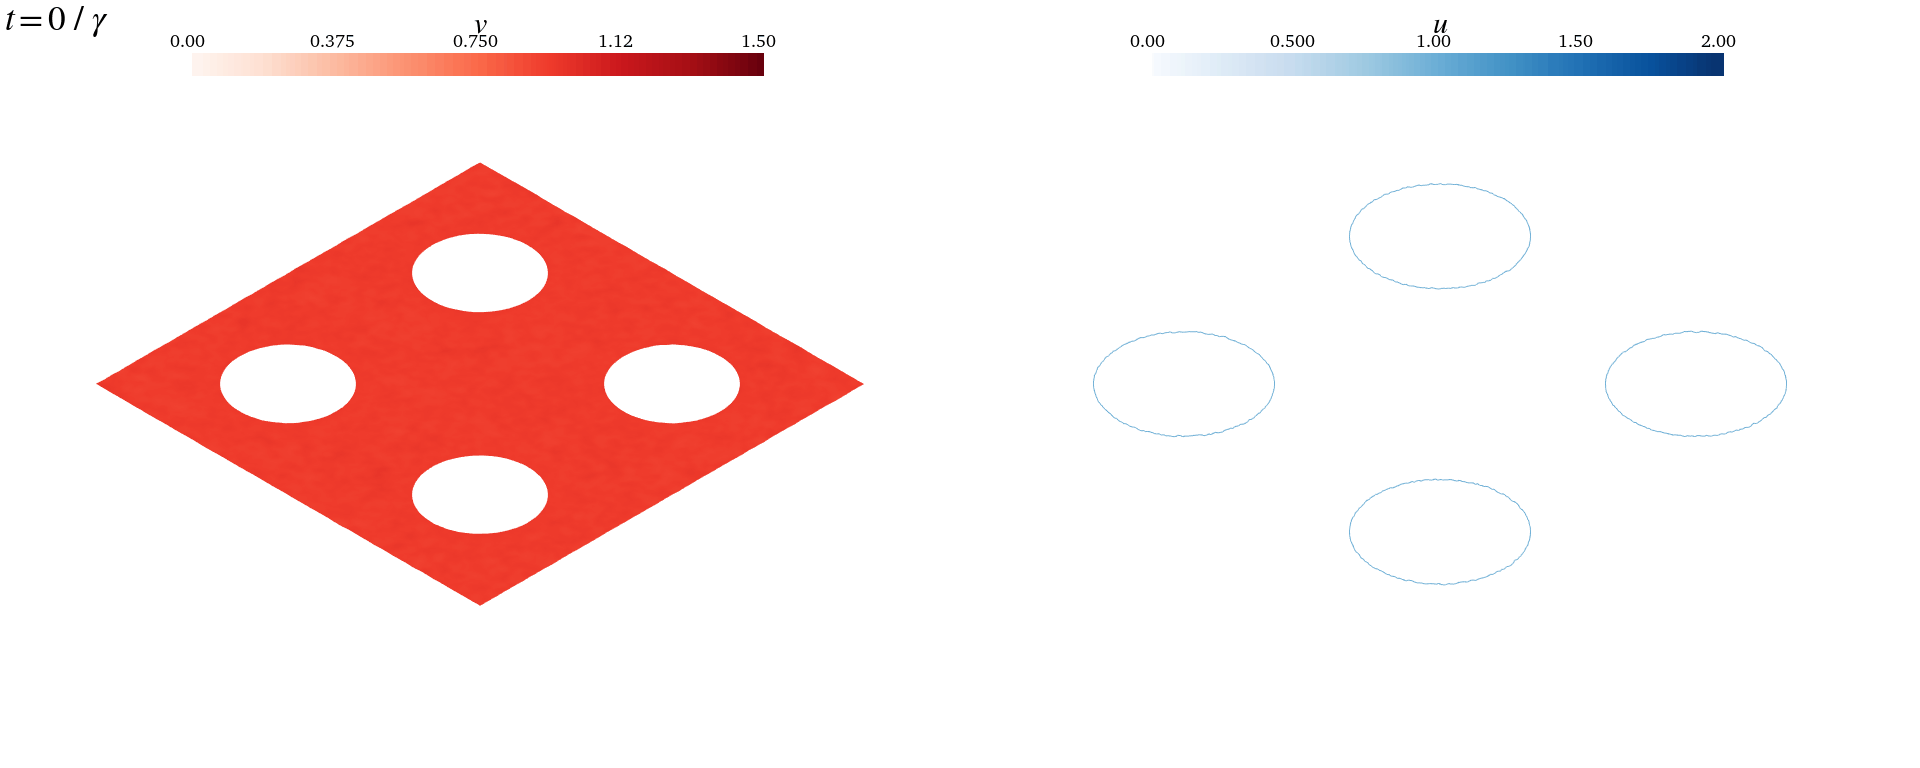
\includegraphics[width=\linewidth]{img/simulation_frames/2d2s_0.png}
    \end{subfigure}

    \vspace{0.4cm}

    \begin{subfigure}{\textwidth}
        \centering
        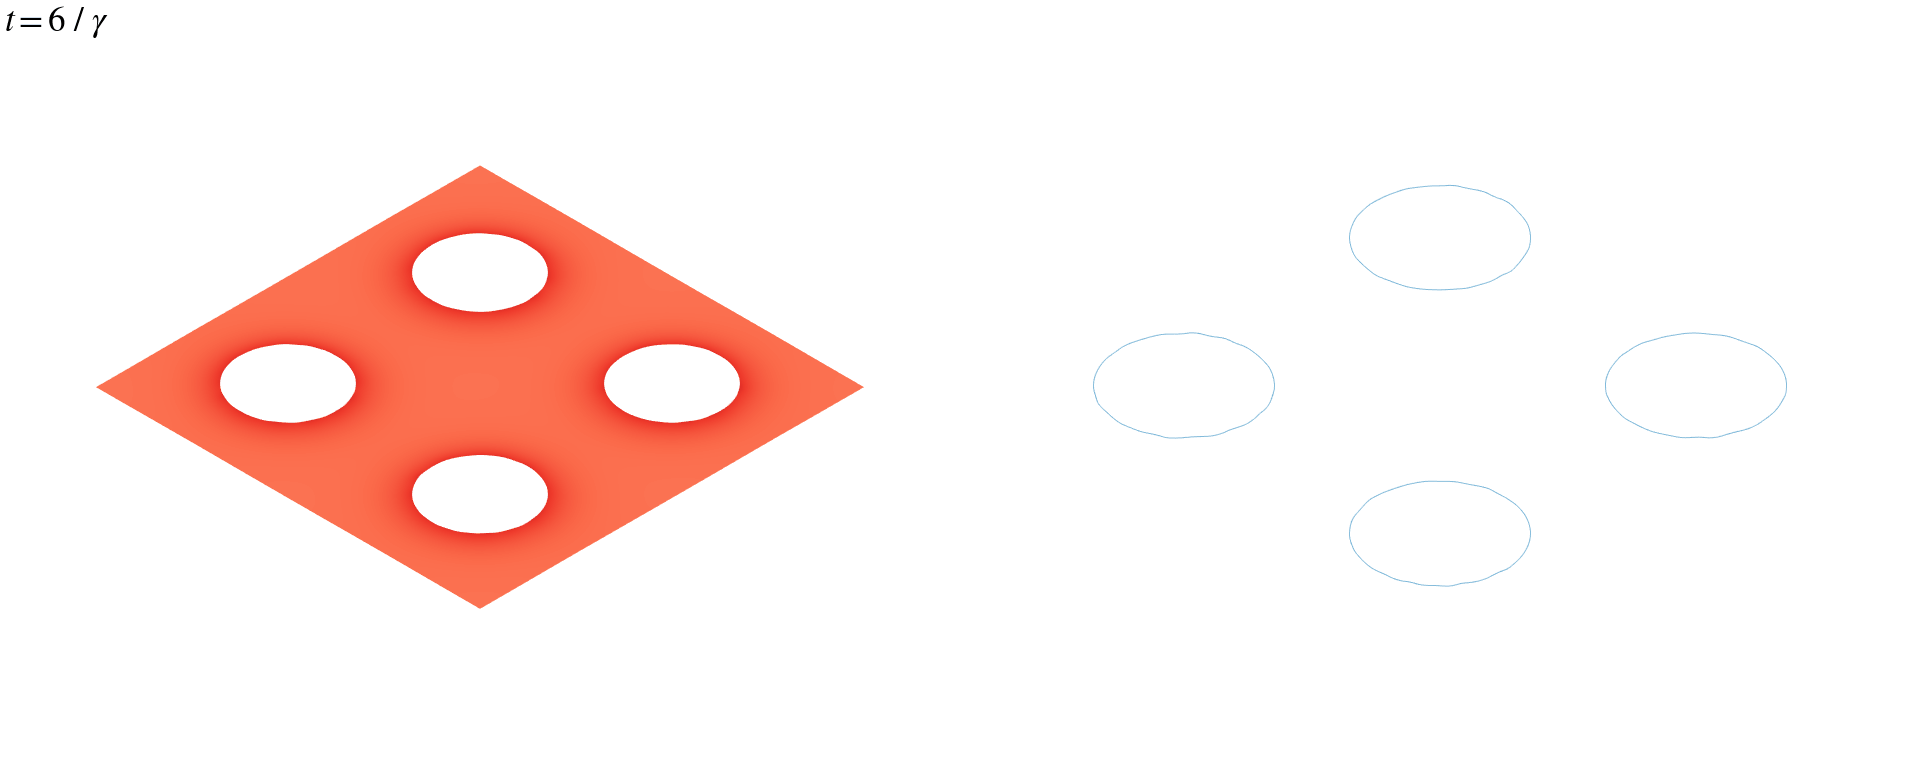
\includegraphics[width=\linewidth]{img/simulation_frames/2d2s_1.png}
    \end{subfigure}

    \vspace{0.4cm}

    \begin{subfigure}{\textwidth}
        \centering
        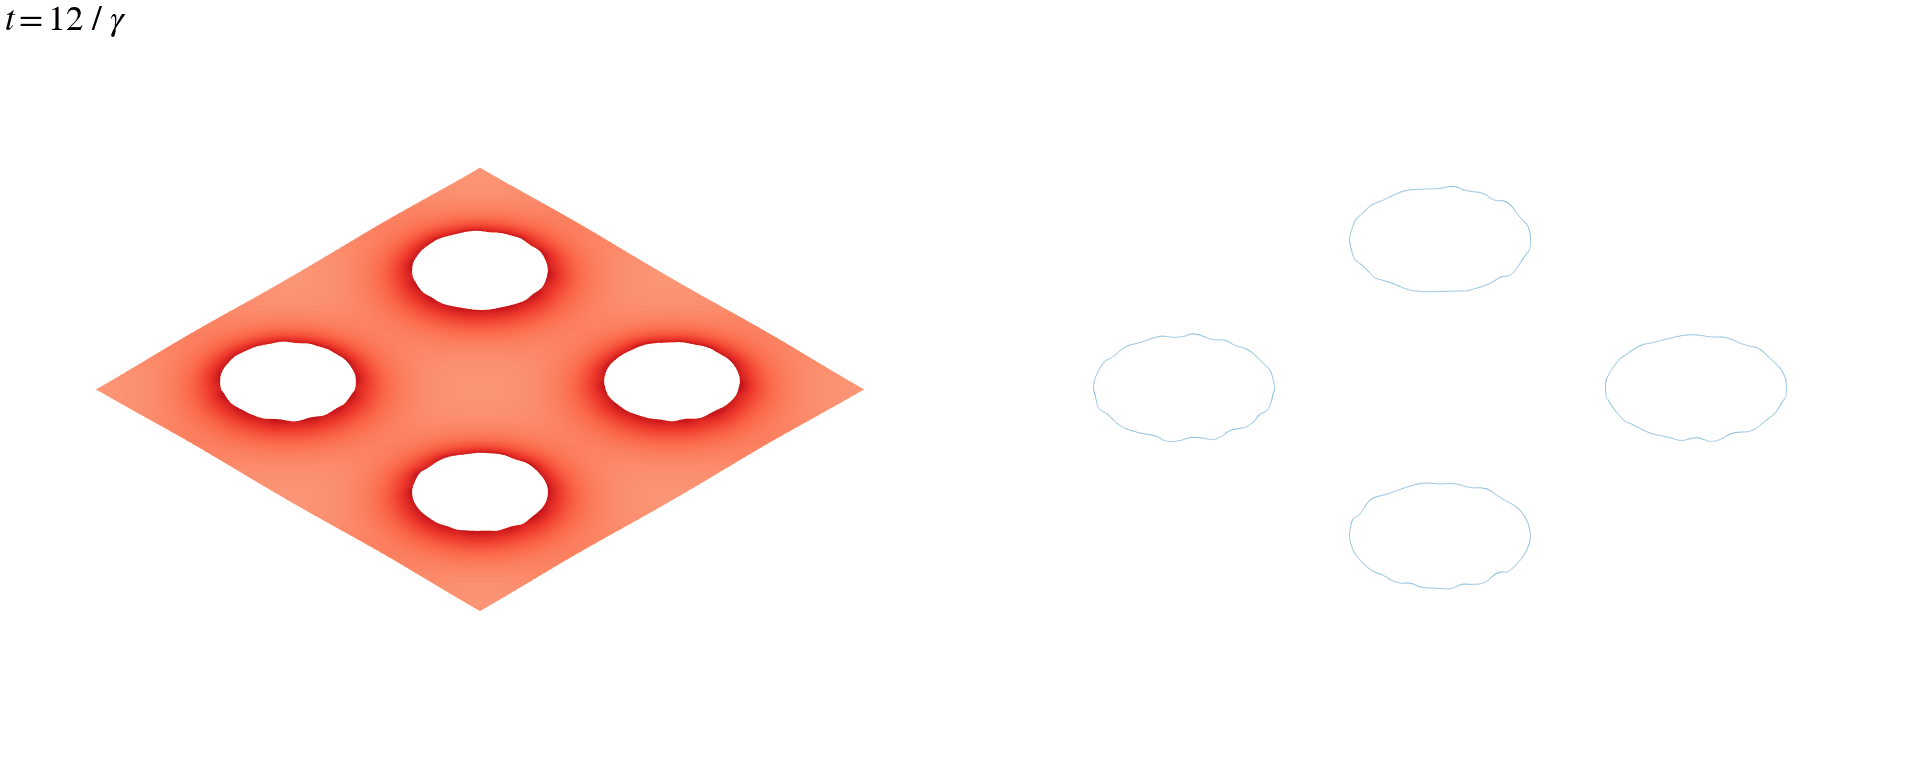
\includegraphics[width=\linewidth]{img/simulation_frames/2d2s_2.png}
    \end{subfigure}

    \caption{A simulation of the Schnakenberg equations with extra decay for $v$ on $\Omega = (-8, 8)^2$ with $\delta_v = 0.1$, $d = 50$, $a = 0.1$, $b = 0.9$ and $\gamma = 12$. The solution is plotted for times $t = 0$, $t = 5/\gamma$ and $t = 11/\gamma$.}
    \label{fig:2d2s_0-2}
\end{figure}

\begin{figure}[t]
    \centering

    \begin{subfigure}{\textwidth}
        \centering
        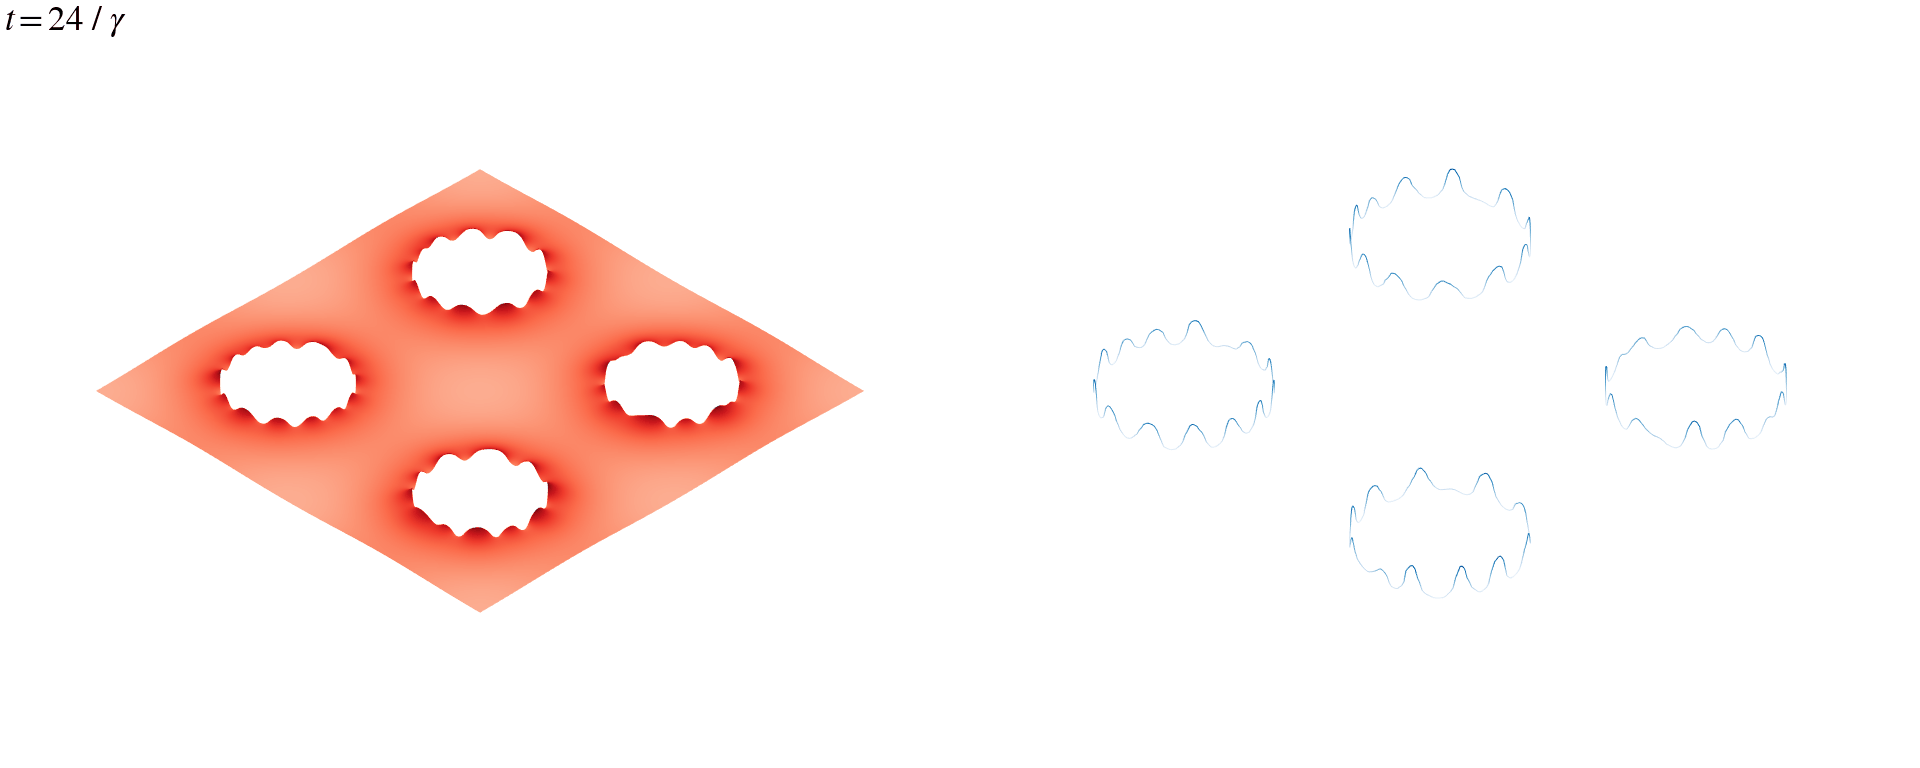
\includegraphics[width=\linewidth]{img/simulation_frames/2d2s_3.png}
    \end{subfigure}

    \vspace{0.4cm}

    \begin{subfigure}{\textwidth}
        \centering
        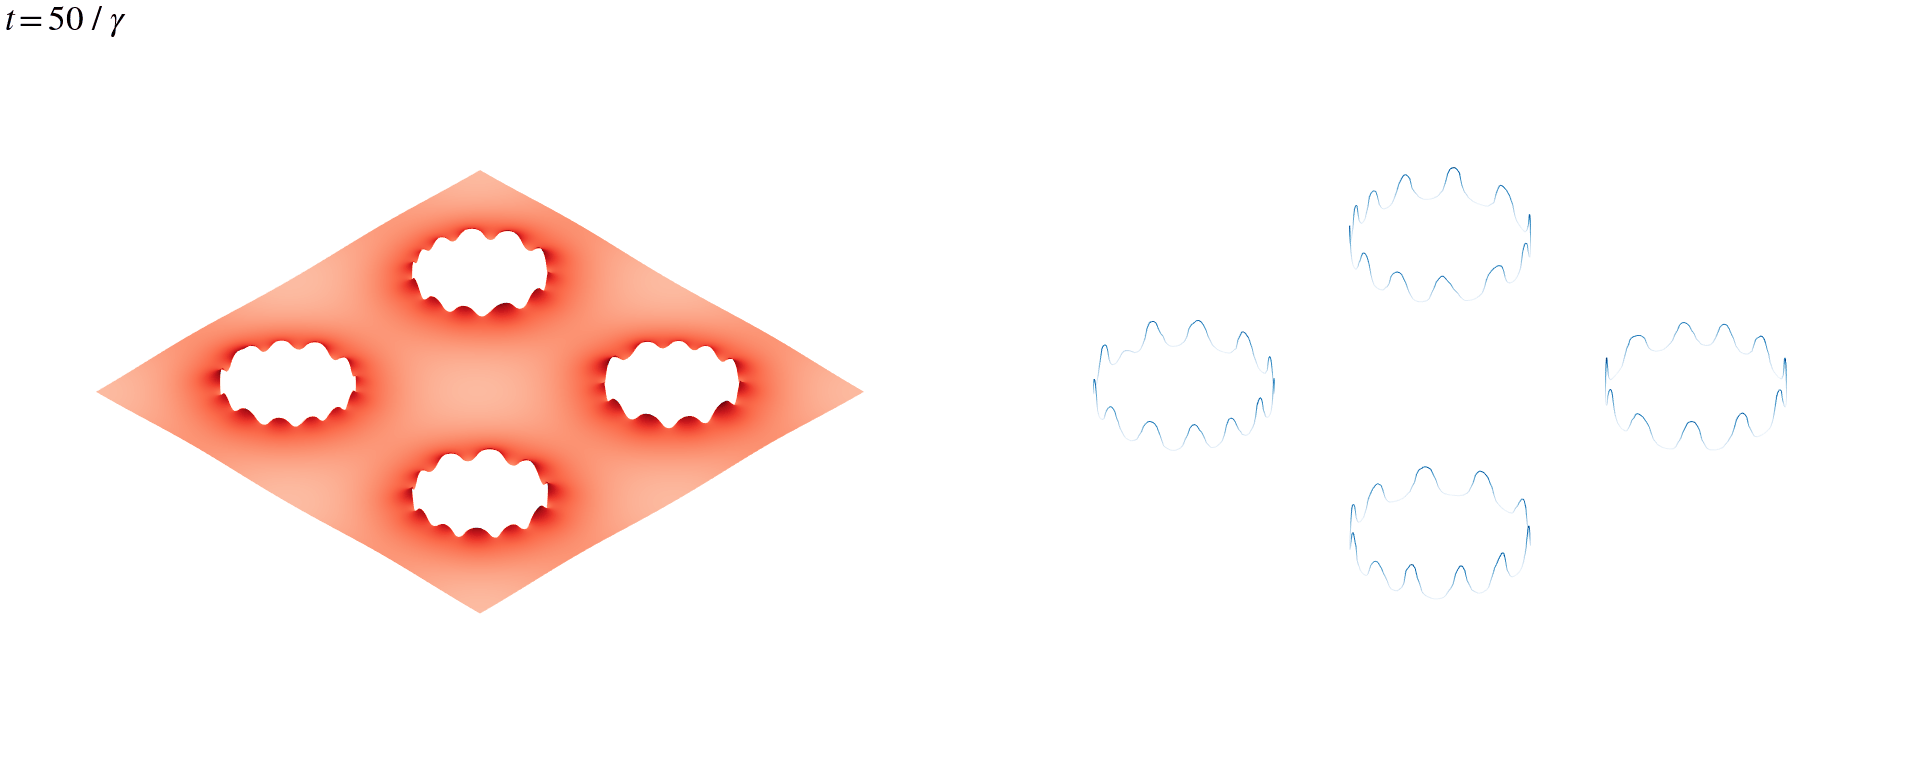
\includegraphics[width=\linewidth]{img/simulation_frames/2d2s_4.png}
    \end{subfigure}

    \vspace{0.4cm}

    \begin{subfigure}{\textwidth}
        \centering
        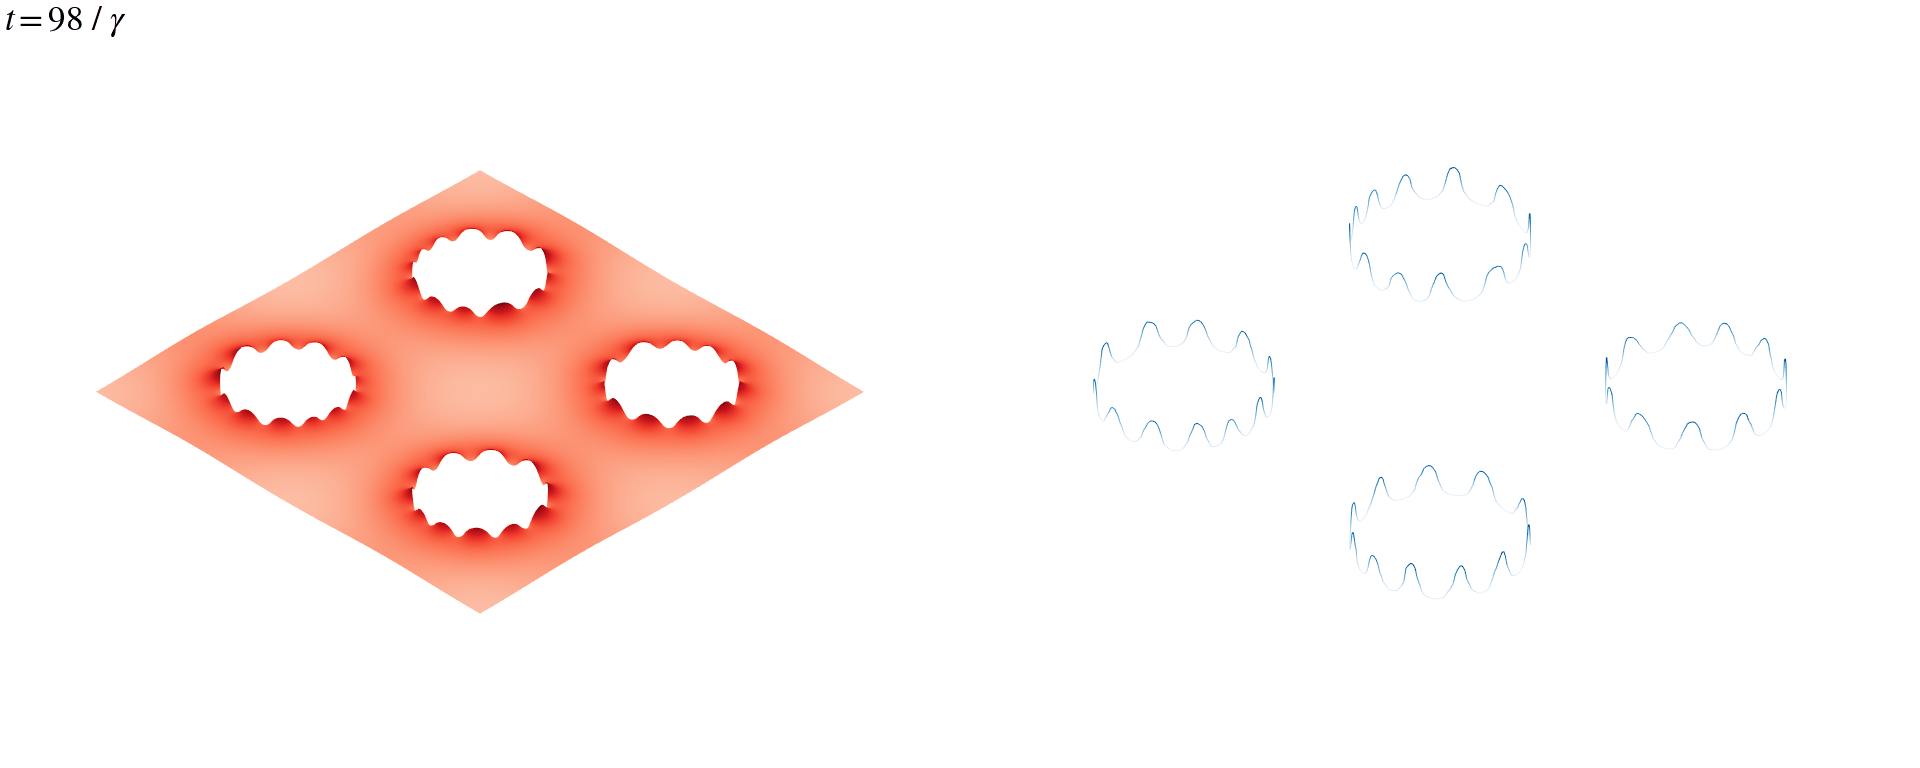
\includegraphics[width=\linewidth]{img/simulation_frames/2d2s_5.png}
    \end{subfigure}

    \caption{A simulation of the Schnakenberg equations with extra decay for $v$ on $\Omega = (-8, 8)^2$ with $\delta_v = 0.1$, $d = 50$, $a = 0.1$, $b = 0.9$ and $\gamma = 12$. The solution is plotted for times $t = 0$, $t = 5/\gamma$ and $t = 11/\gamma$.}
    \label{fig:2d2s_3-5}
\end{figure}

We compare this to the numerical solutions of \cref{eq:threespeciesmodel}. To simulate the quasi-steady state assumption, we set $\kappa = 50$. This necessitates increasing the number of steps $N$ significantly to preserve numerical stability. If the model of two species proves to be a good representation of the three-species model, it would be preferable to use this model rather than the full three-species equivalent, since it is simpler to analyse both numerically and analytically. In \cref{fig:2d3s_0-2,fig:2d3s_3-5}, the numerical solution of \cref{eq:threespeciesmodel} is plotted for similar time steps. It admits the same general behaviour as the numerical solution of \cref{eq:twospeciesmodel}, smoothing out the perturbations before forming Turing patterns of similar scale and shape. The patterns formed by $u$ and $u_b$ almost coincide, with the peaks of $u_b$ being a slightly higher than those of $u$. This can be justified by the extra scaling coefficient $\kappa$ dominating the diffusion.

\begin{figure}[t]
    \centering

    \begin{subfigure}{\textwidth}
        \centering
        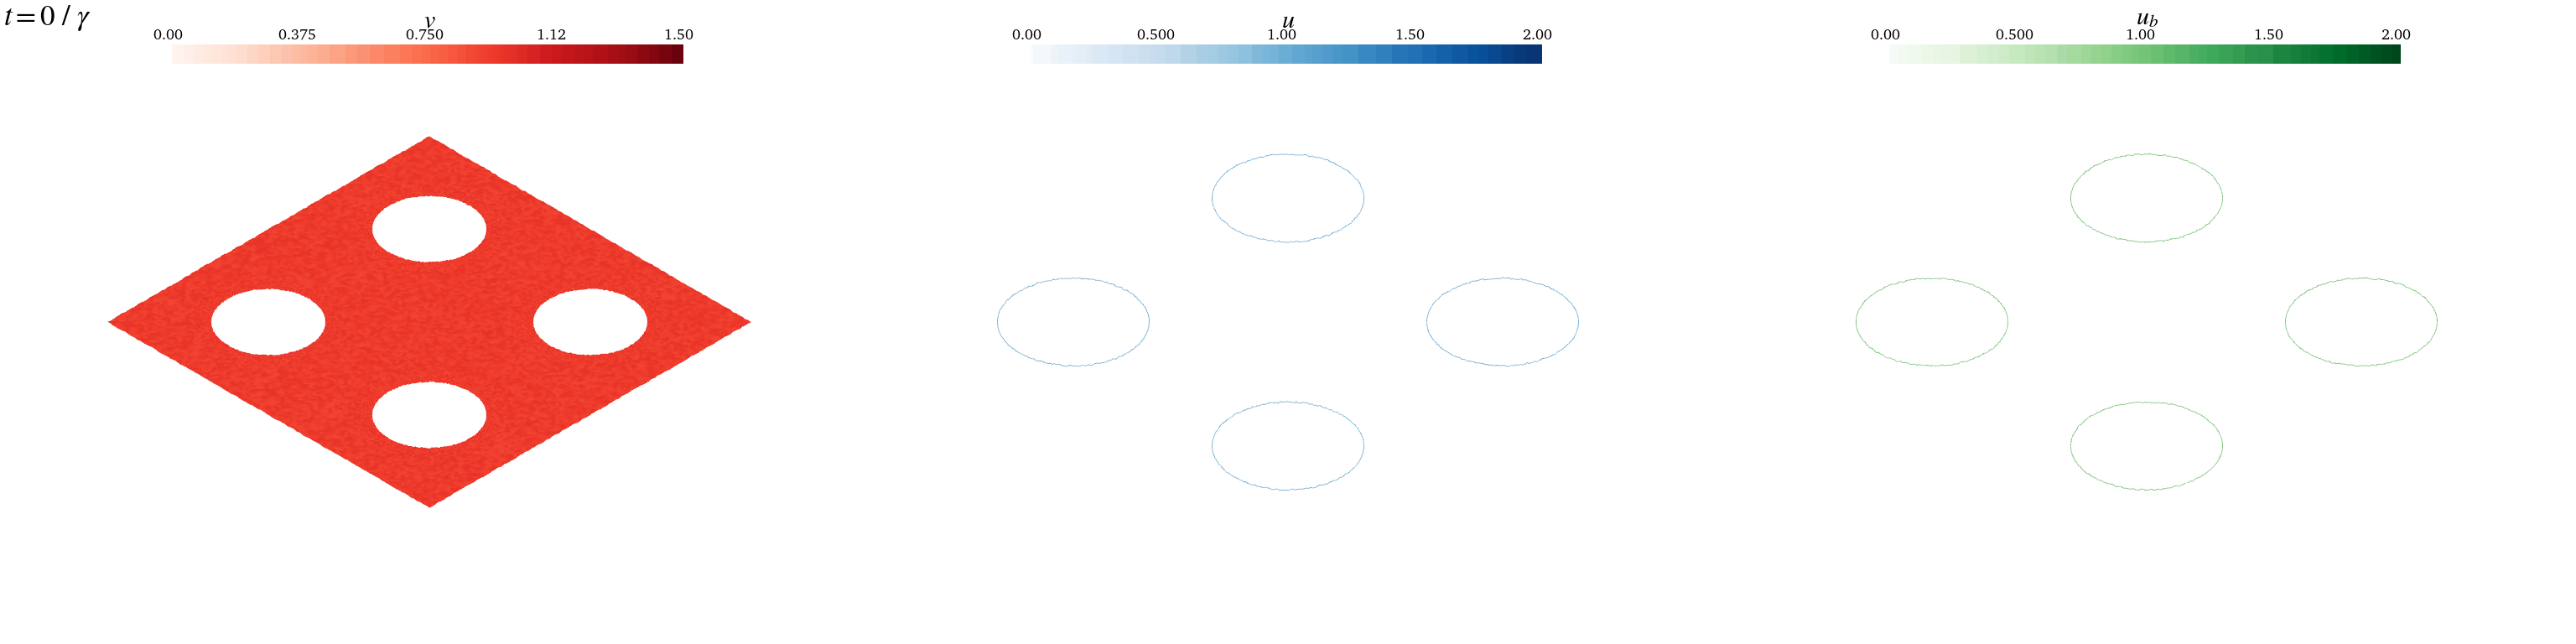
\includegraphics[width=\linewidth]{img/simulation_frames/2d3s_0.png}
    \end{subfigure}

    \vspace{0.4cm}

    \begin{subfigure}{\textwidth}
        \centering
        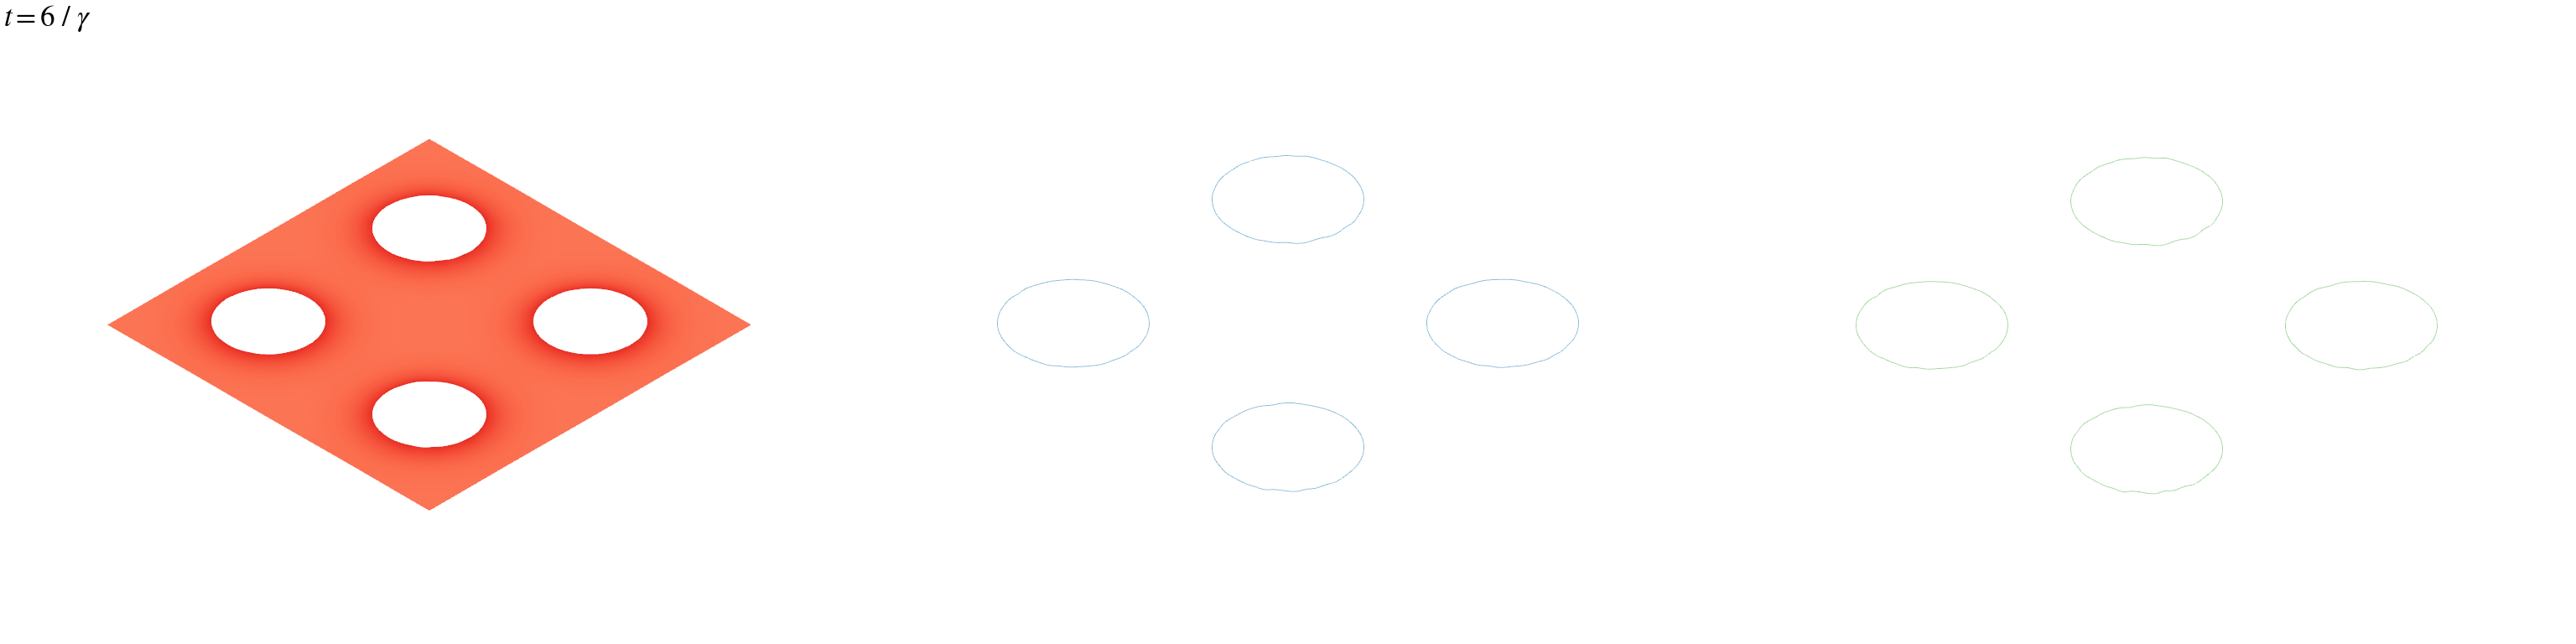
\includegraphics[width=\linewidth]{img/simulation_frames/2d3s_1.png}
    \end{subfigure}

    \vspace{0.4cm}

    \begin{subfigure}{\textwidth}
        \centering
        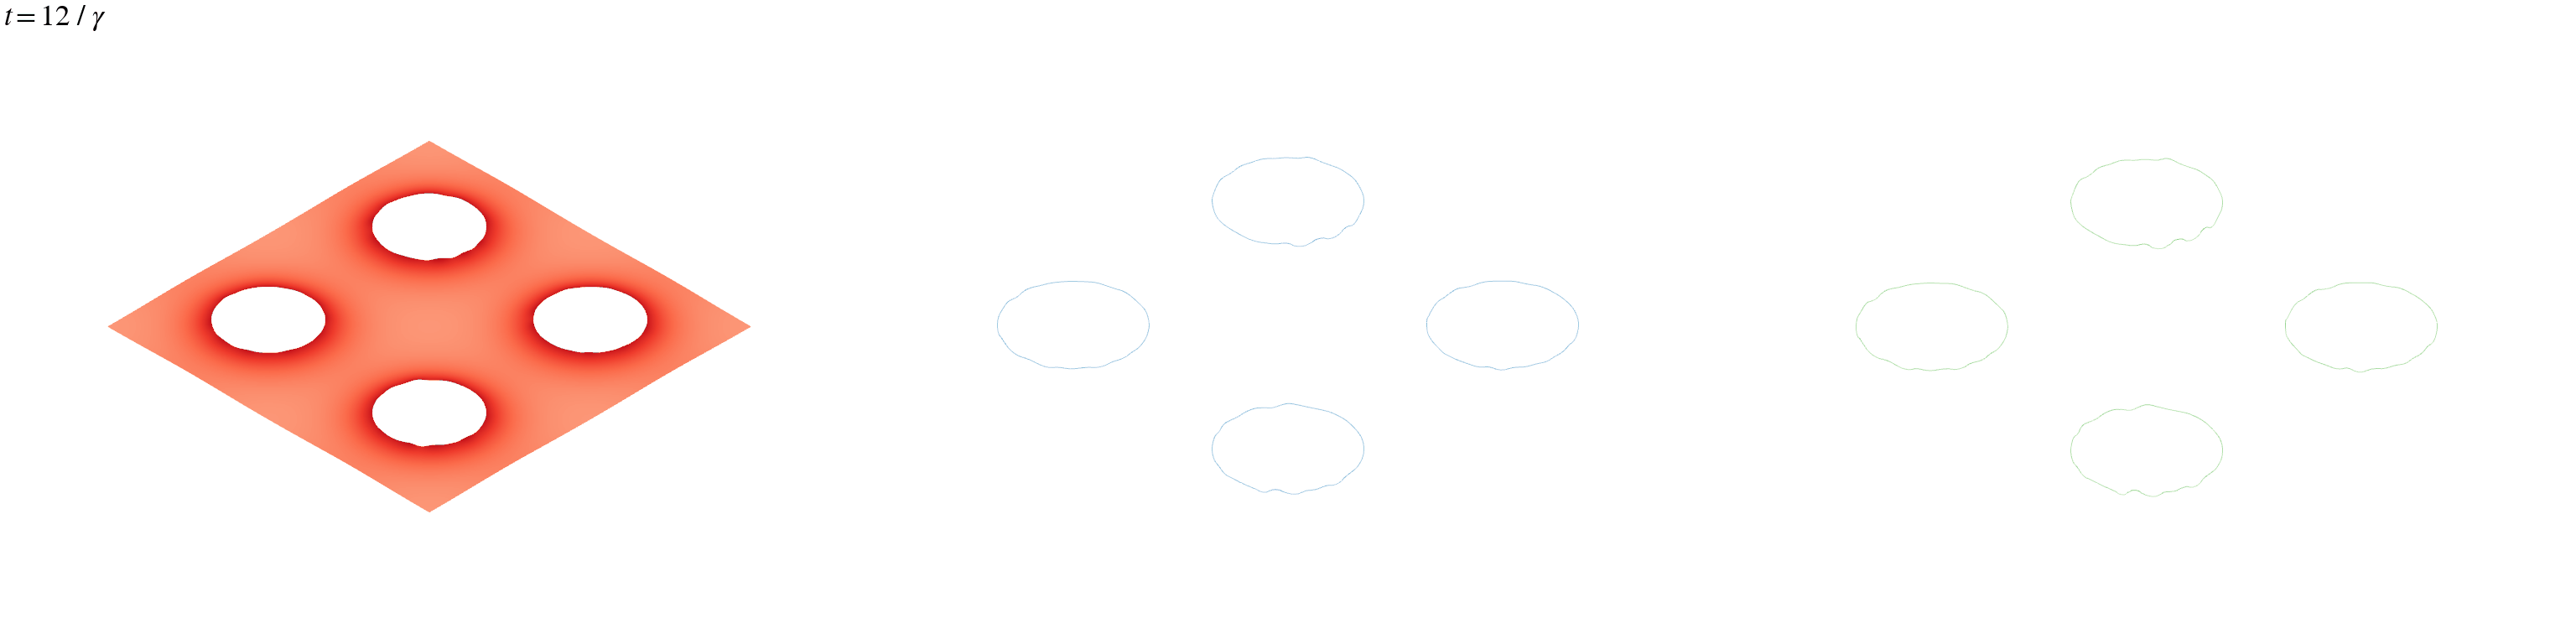
\includegraphics[width=\linewidth]{img/simulation_frames/2d3s_2.png}
    \end{subfigure}

    \caption{A simulation of the Schnakenberg equations with extra decay for $v$ on $\Omega = (-8, 8)^2$ with $\delta_v = 0.1$, $d = 50$, $a = 0.1$, $b = 0.9$ and $\gamma = 12$. The solution is plotted for times $t = 0$, $t = 5/\gamma$ and $t = 11/\gamma$.}
    \label{fig:2d3s_0-2}
\end{figure}

\begin{figure}[t]
    \centering

    \begin{subfigure}{\textwidth}
        \centering
        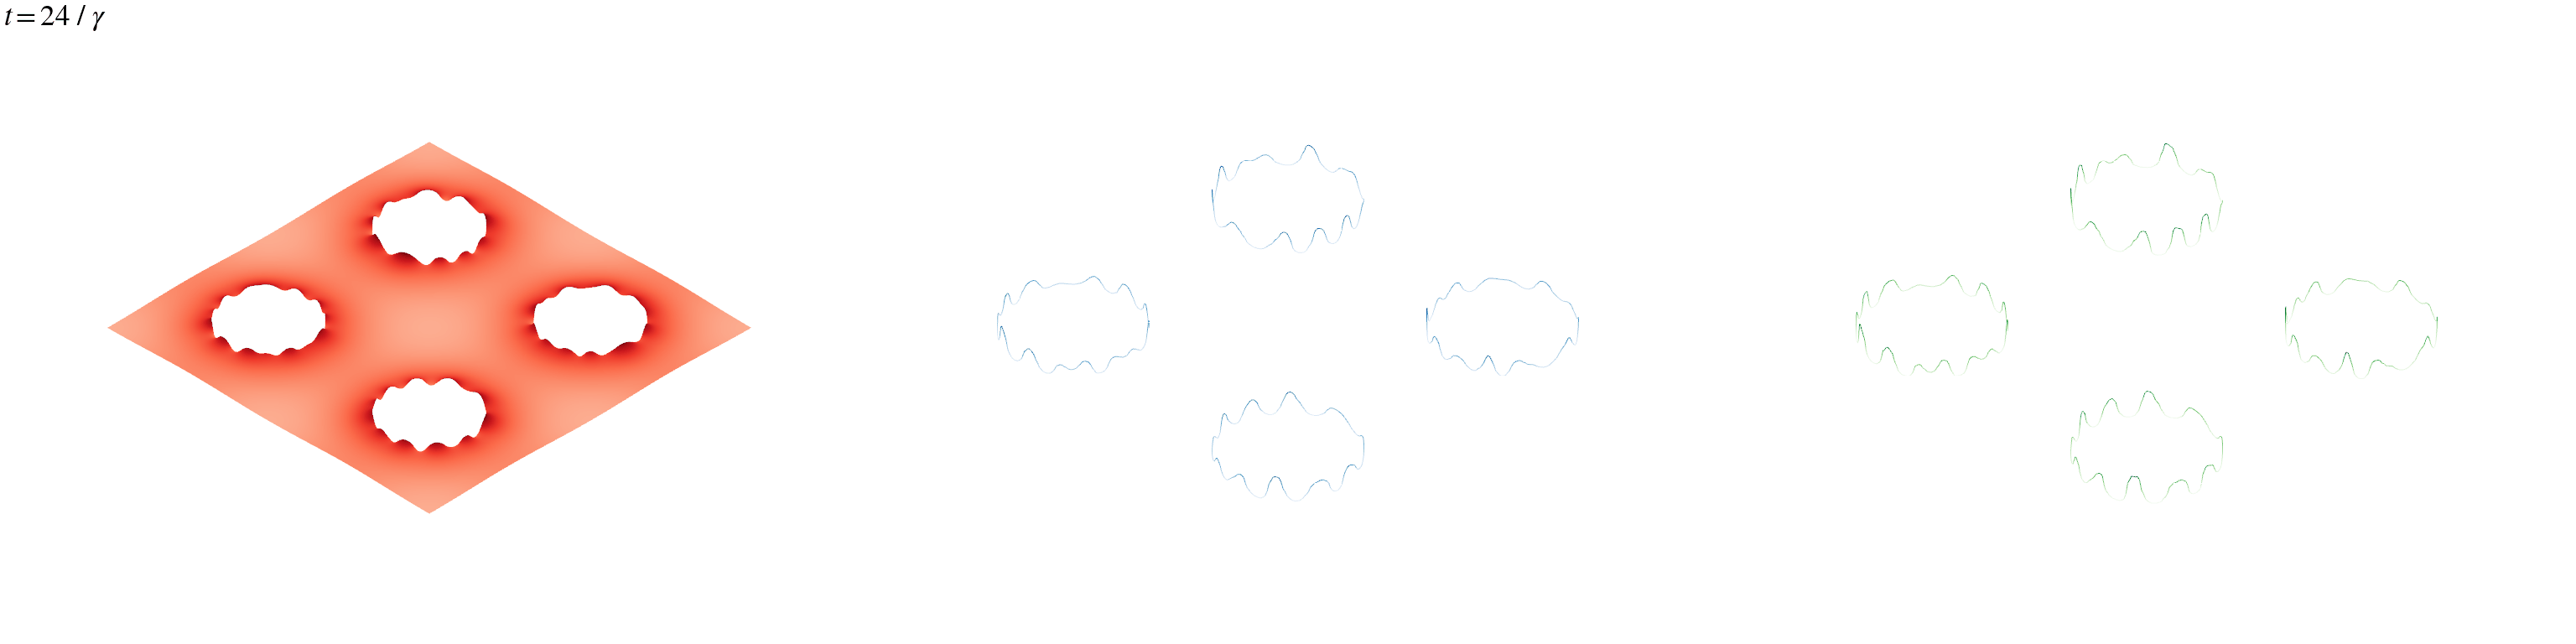
\includegraphics[width=\linewidth]{img/simulation_frames/2d3s_3.png}
    \end{subfigure}

    \vspace{0.4cm}

    \begin{subfigure}{\textwidth}
        \centering
        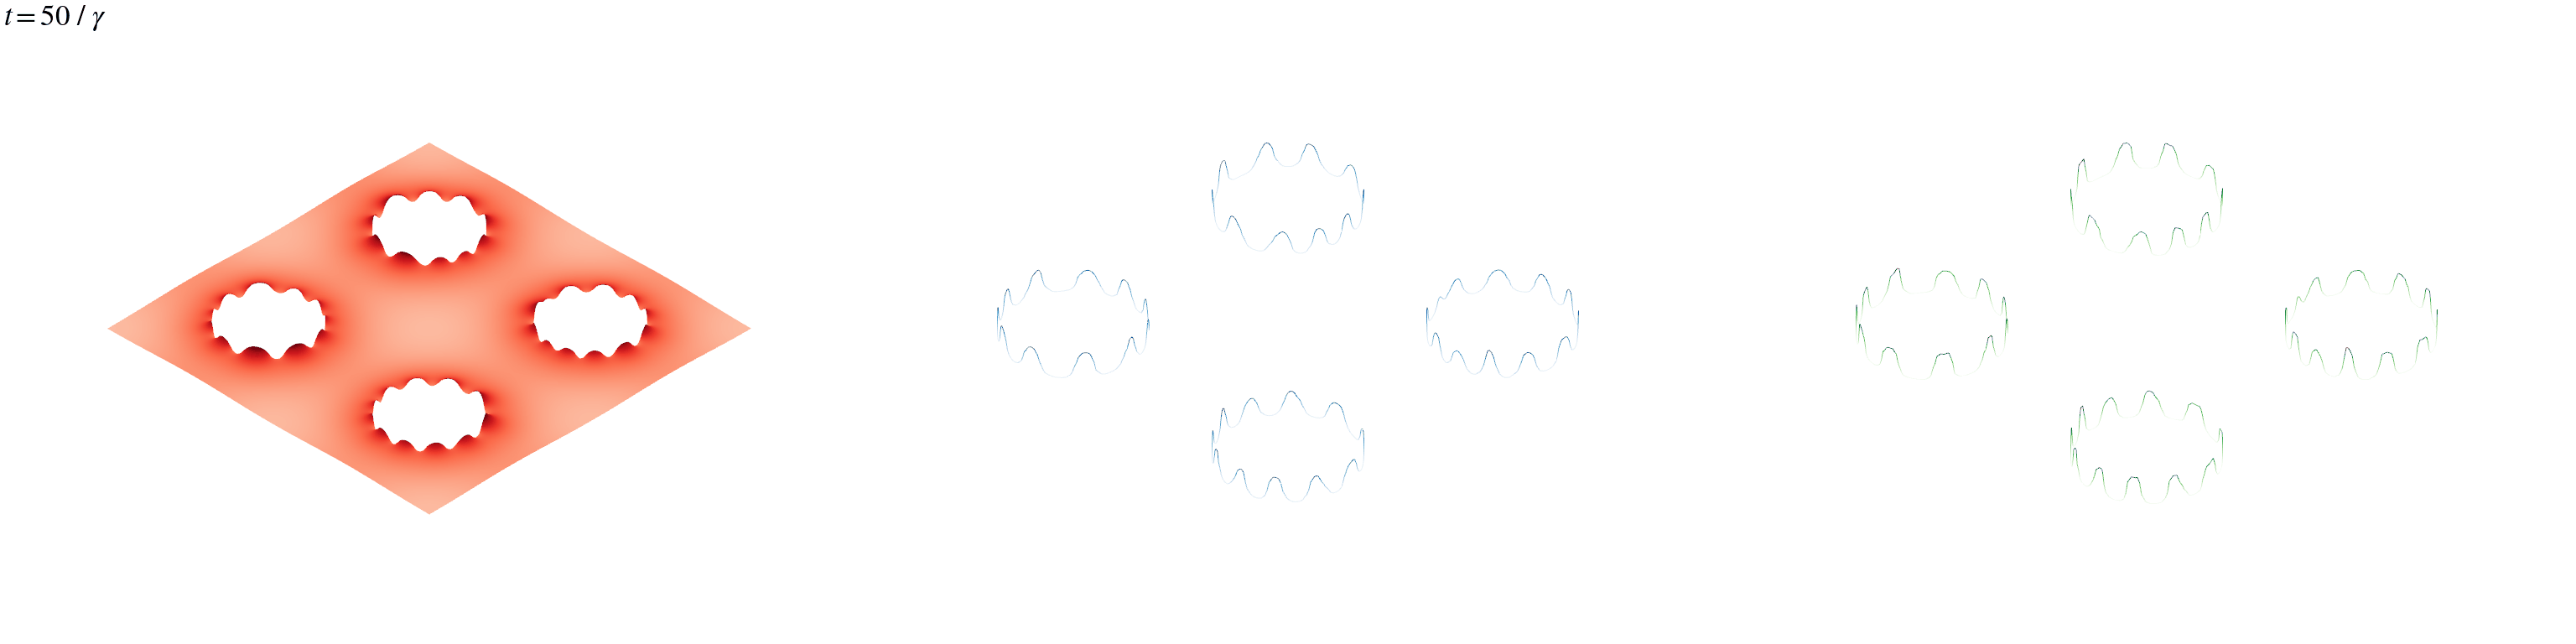
\includegraphics[width=\linewidth]{img/simulation_frames/2d3s_4.png}
    \end{subfigure}

    \vspace{0.4cm}

    \begin{subfigure}{\textwidth}
        \centering
        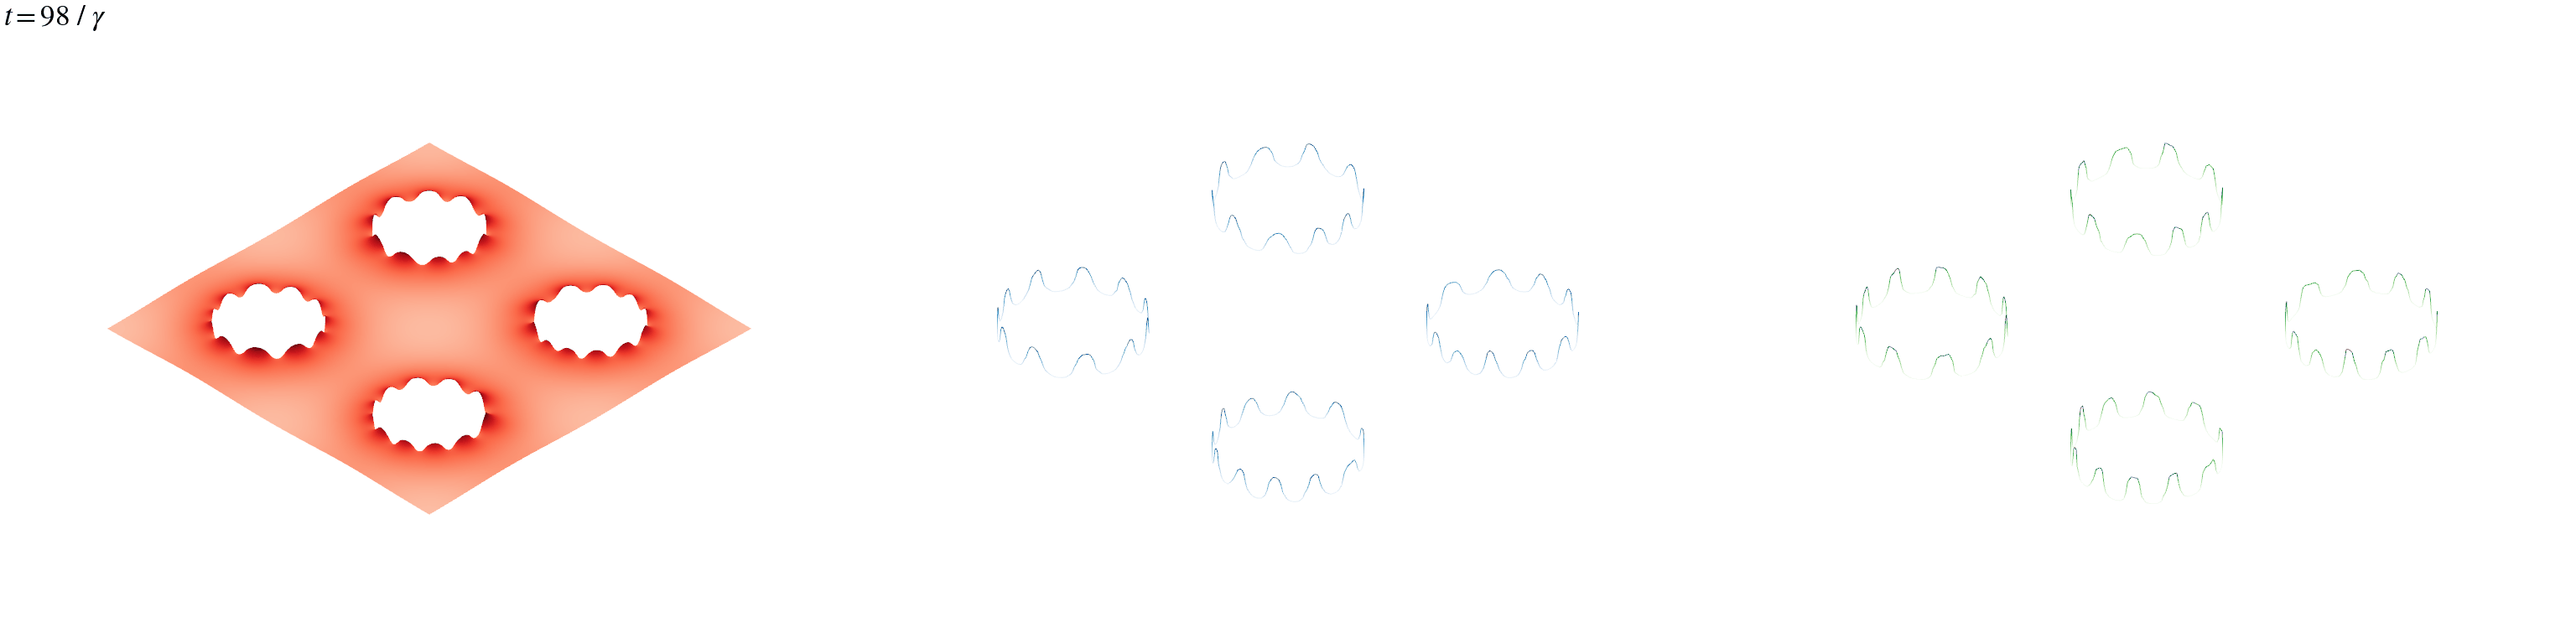
\includegraphics[width=\linewidth]{img/simulation_frames/2d3s_5.png}
    \end{subfigure}

    \caption{A simulation of the Schnakenberg equations with extra decay for $v$ on $\Omega = (-8, 8)^2$ with $\delta_v = 0.1$, $d = 50$, $a = 0.1$, $b = 0.9$ and $\gamma = 12$. The solution is plotted for times $t = 0$, $t = 5/\gamma$ and $t = 11/\gamma$.}
    \label{fig:2d3s_3-5}
\end{figure}

For $d = 3$, the domain is defined as the open cube $(-16, 16)^3$ without the eight closed spheres of radius $4$ and centers $(\pm 8, \pm 8, \pm 8)$, and $\Gamma$ is defined as the boundary of these spheres. In \cref{fig:3d2s_0-2,fig:3d2s_3-5}, we see the two-species system form patterns on the cell membranes and their effect on the concentration of ligands in the immediate neighbourhood of the cell membranes. Again, this behaviour is very similar to the numerical solution of the three-species model, shown in \cref{fig:3d3s_0-2,fig:3d3s_3-5}. The peaks of $u$ are also similar to that of $u_b$ again, with the peaks of $u_b$ being slightly higher than those of $u$.

\begin{figure}[t]
    \centering

    \begin{subfigure}{\textwidth}
        \centering
        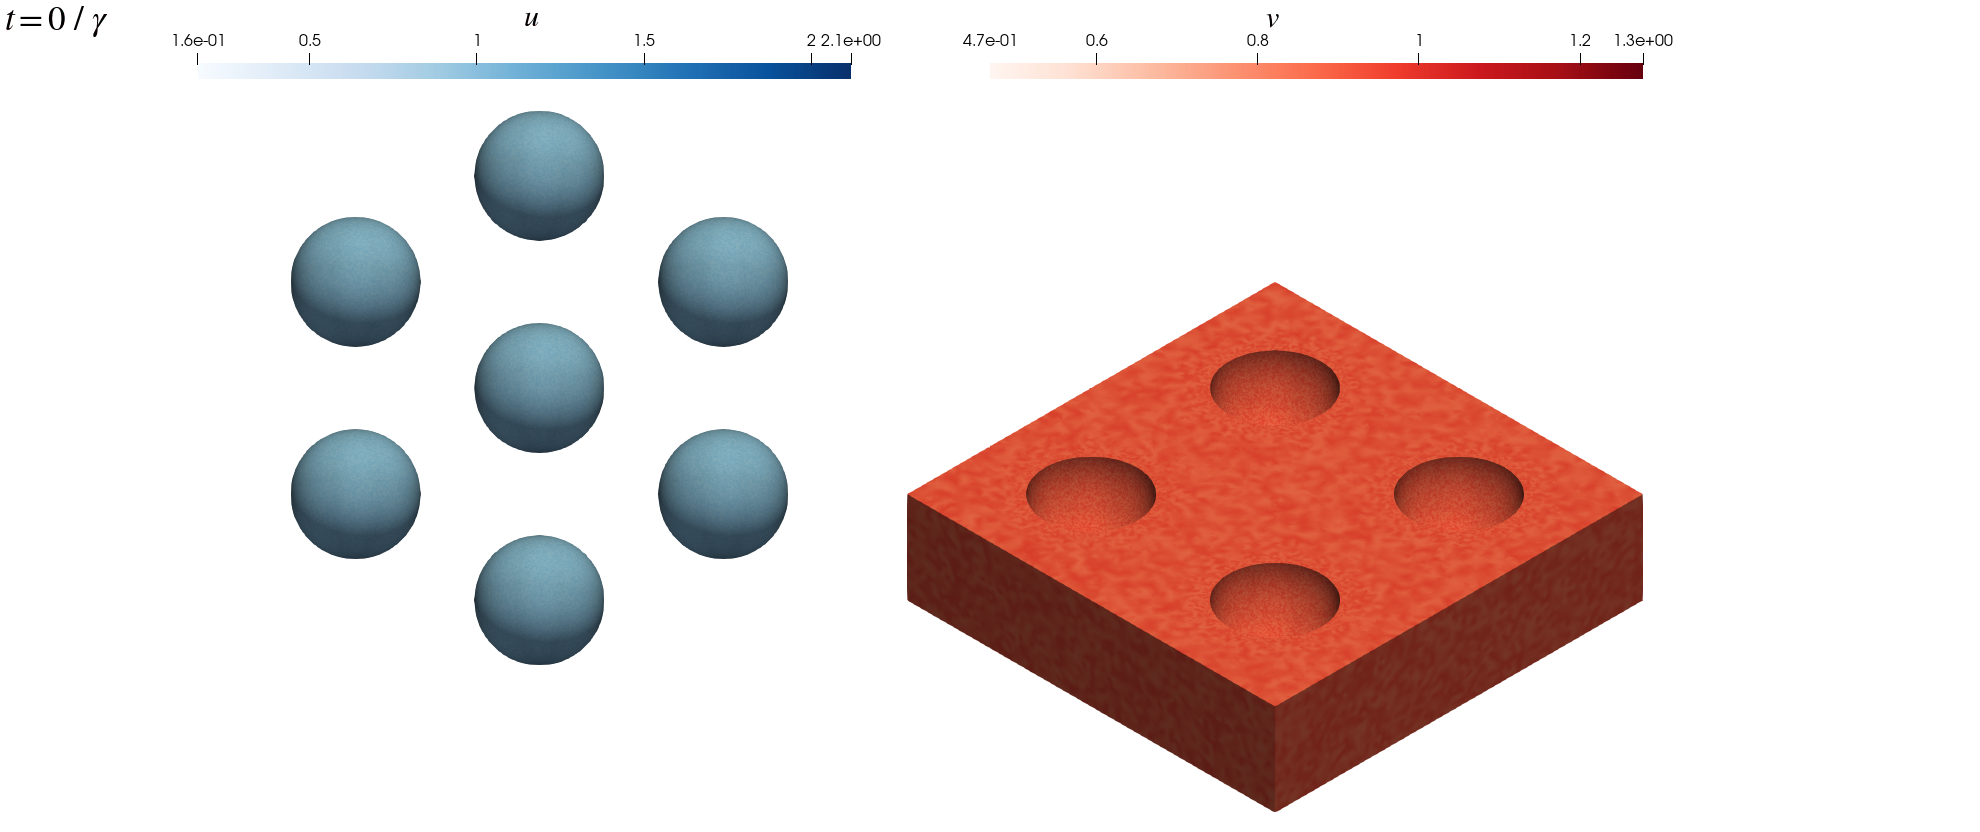
\includegraphics[width=\linewidth]{img/simulation_frames/3dbs2s_2.0000.png}
    \end{subfigure}

    \vspace{0.4cm}

    \begin{subfigure}{\textwidth}
        \centering
        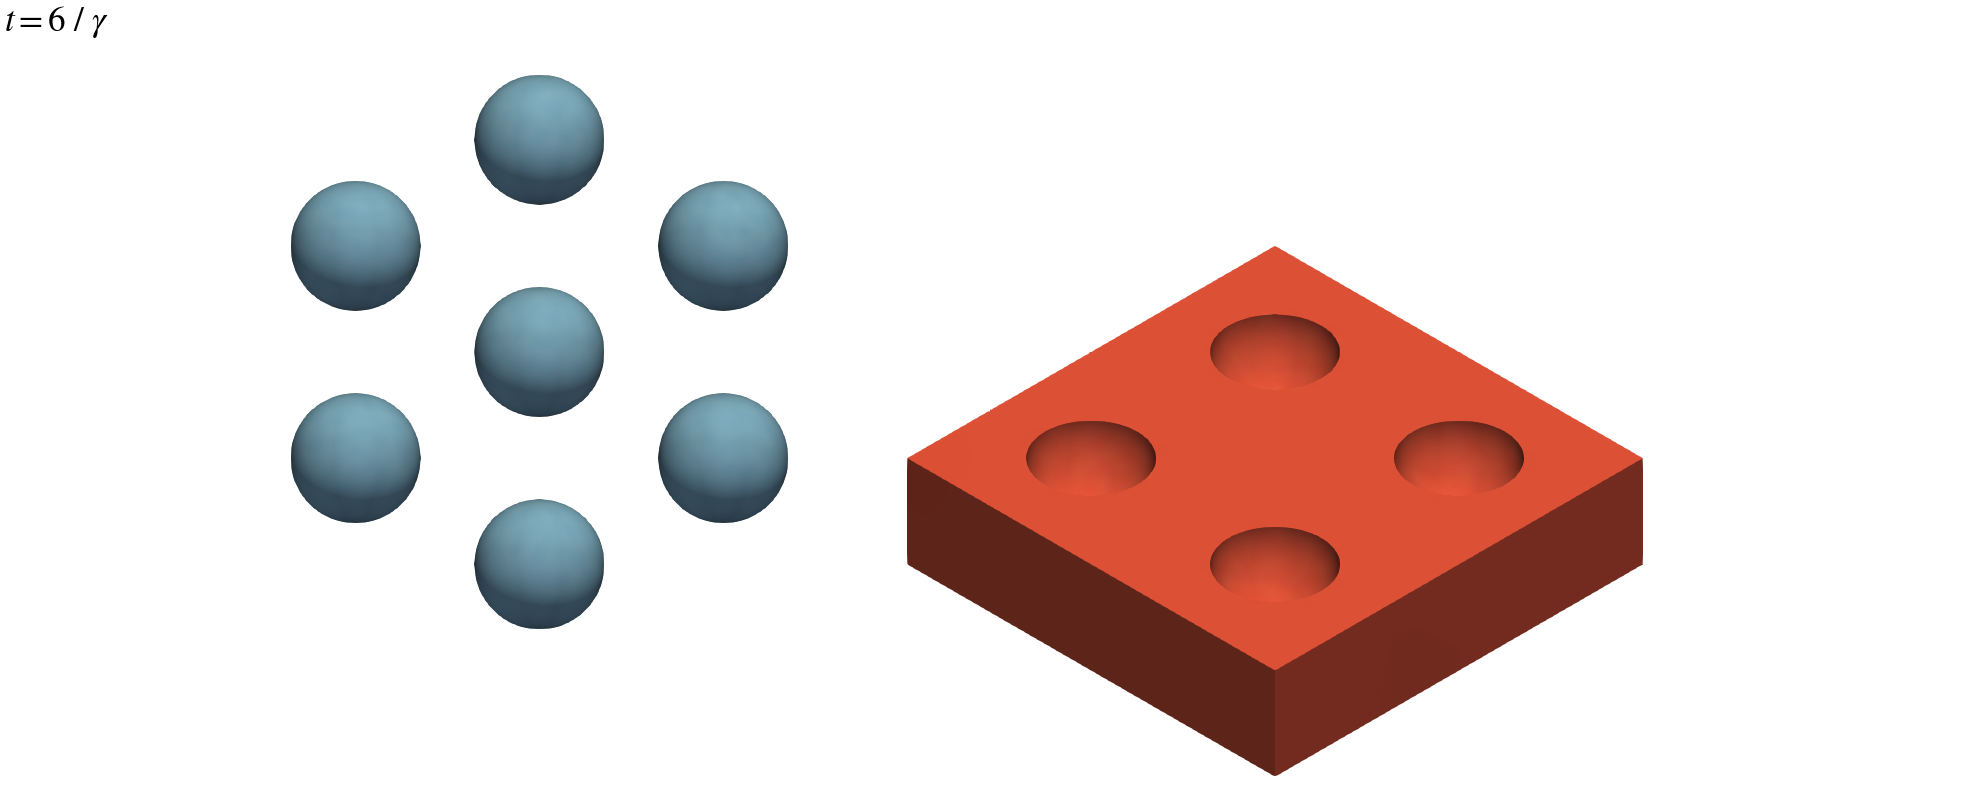
\includegraphics[width=\linewidth]{img/simulation_frames/3dbs2s_2.0008.png}
    \end{subfigure}

    \vspace{0.4cm}

    \begin{subfigure}{\textwidth}
        \centering
        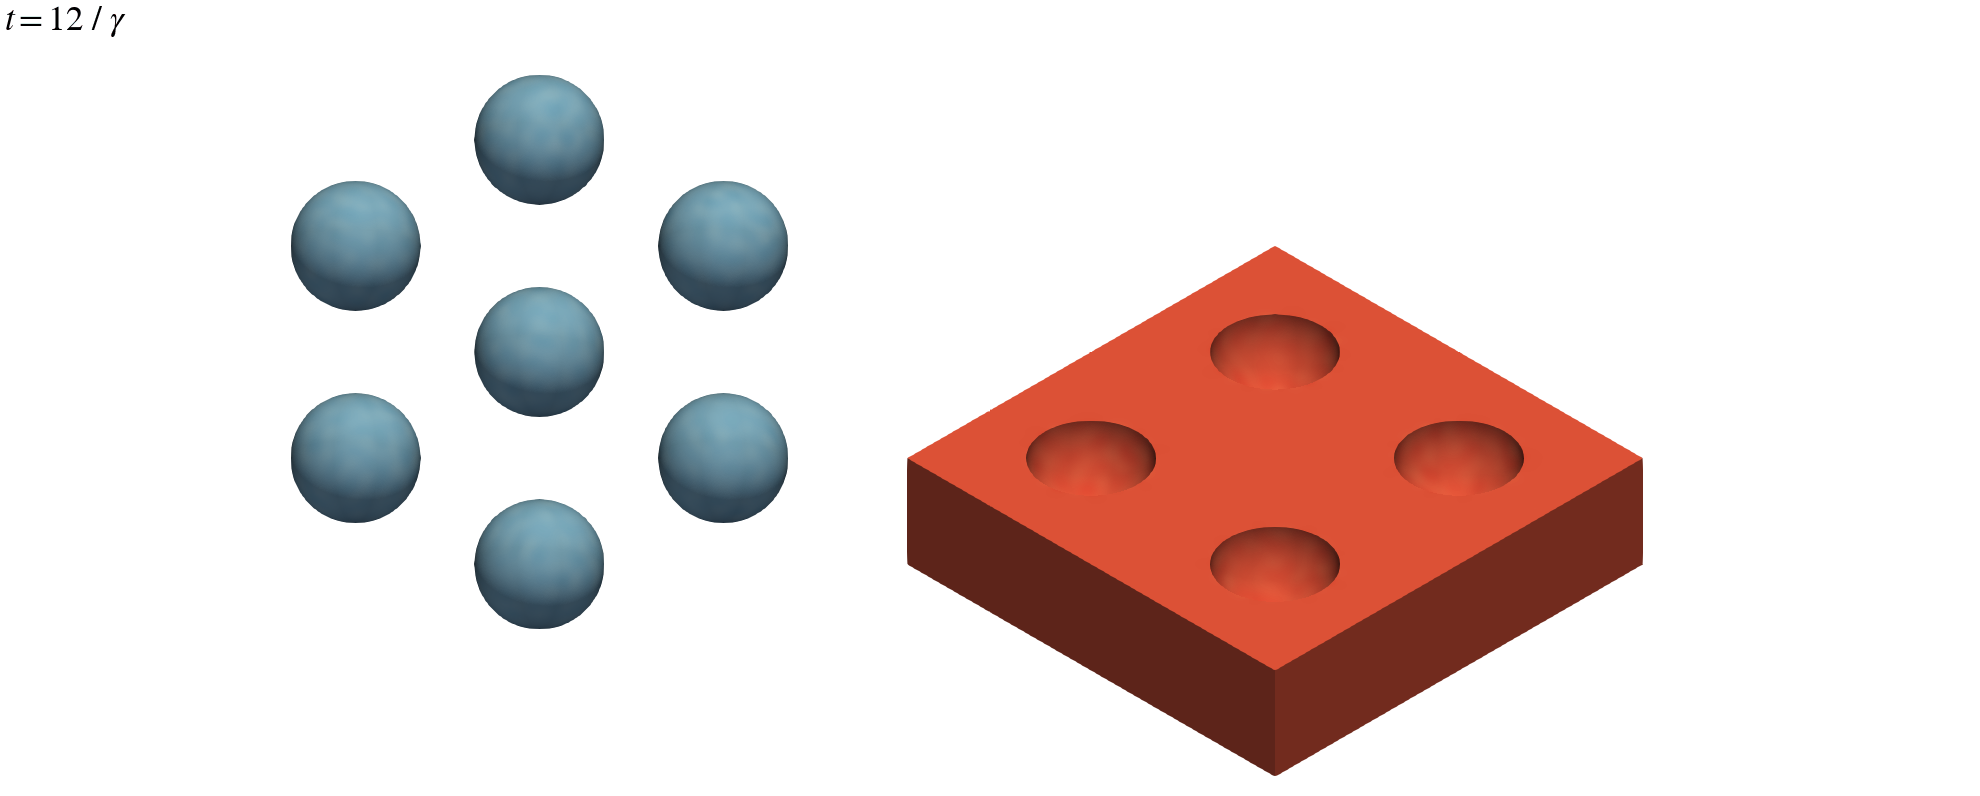
\includegraphics[width=\linewidth]{img/simulation_frames/3dbs2s_2.0016.png}
    \end{subfigure}

    \caption{A simulation of the Schnakenberg equations with extra decay for $v$ on $\Omega = (-8, 8)^2$ with $\delta_v = 0.1$, $d = 50$, $a = 0.1$, $b = 0.9$ and $\gamma = 12$. The solution is plotted for times $t = 0$, $t = 5/\gamma$ and $t = 11/\gamma$.}
    \label{fig:3d2s_0-2}
\end{figure}

\begin{figure}[t]
    \centering

    \begin{subfigure}{\textwidth}
        \centering
        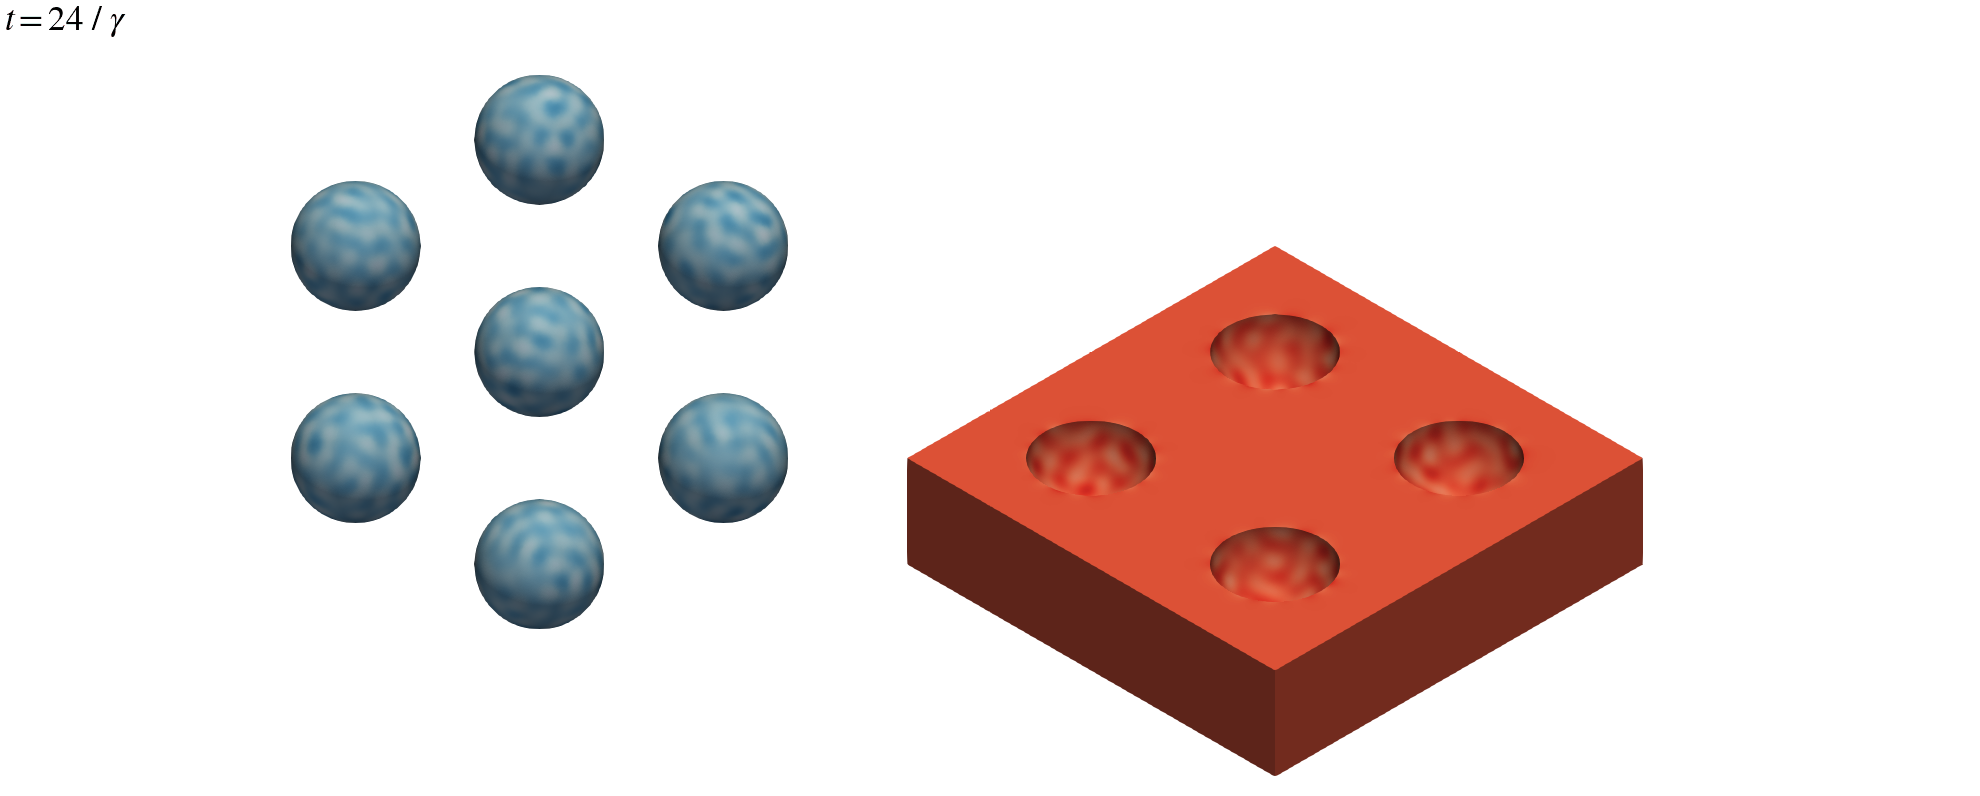
\includegraphics[width=\linewidth]{img/simulation_frames/3dbs2s_2.0032.png}
    \end{subfigure}

    \vspace{0.4cm}

    \begin{subfigure}{\textwidth}
        \centering
        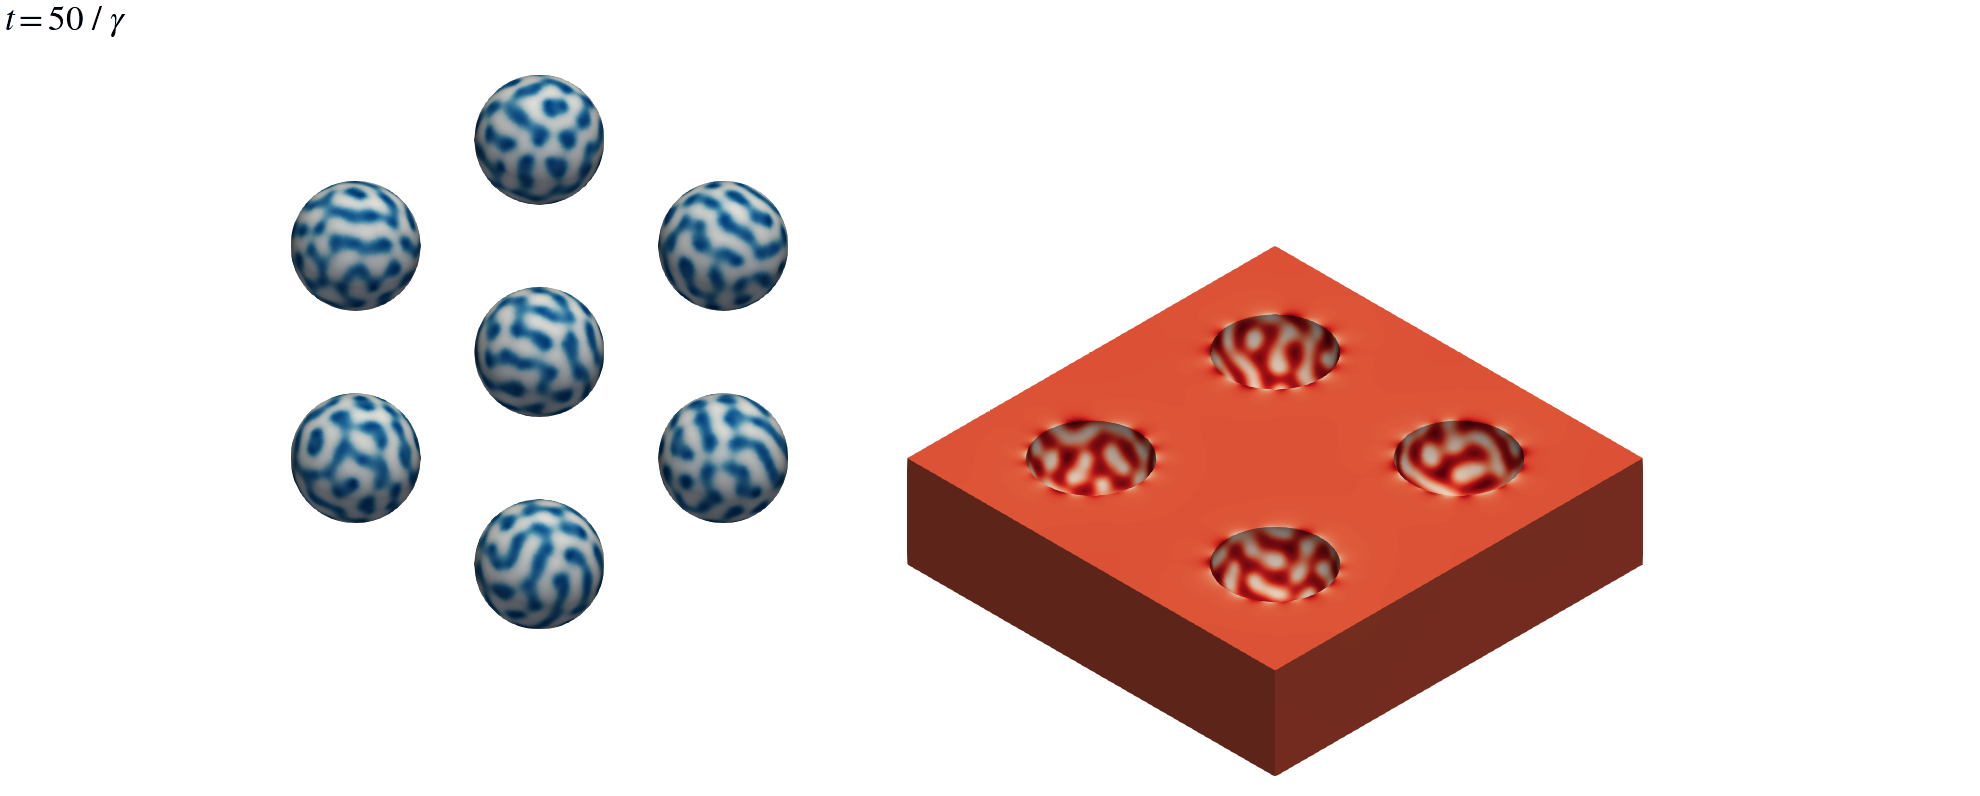
\includegraphics[width=\linewidth]{img/simulation_frames/3dbs2s_2.0064.png}
    \end{subfigure}

    \vspace{0.4cm}

    \begin{subfigure}{\textwidth}
        \centering
        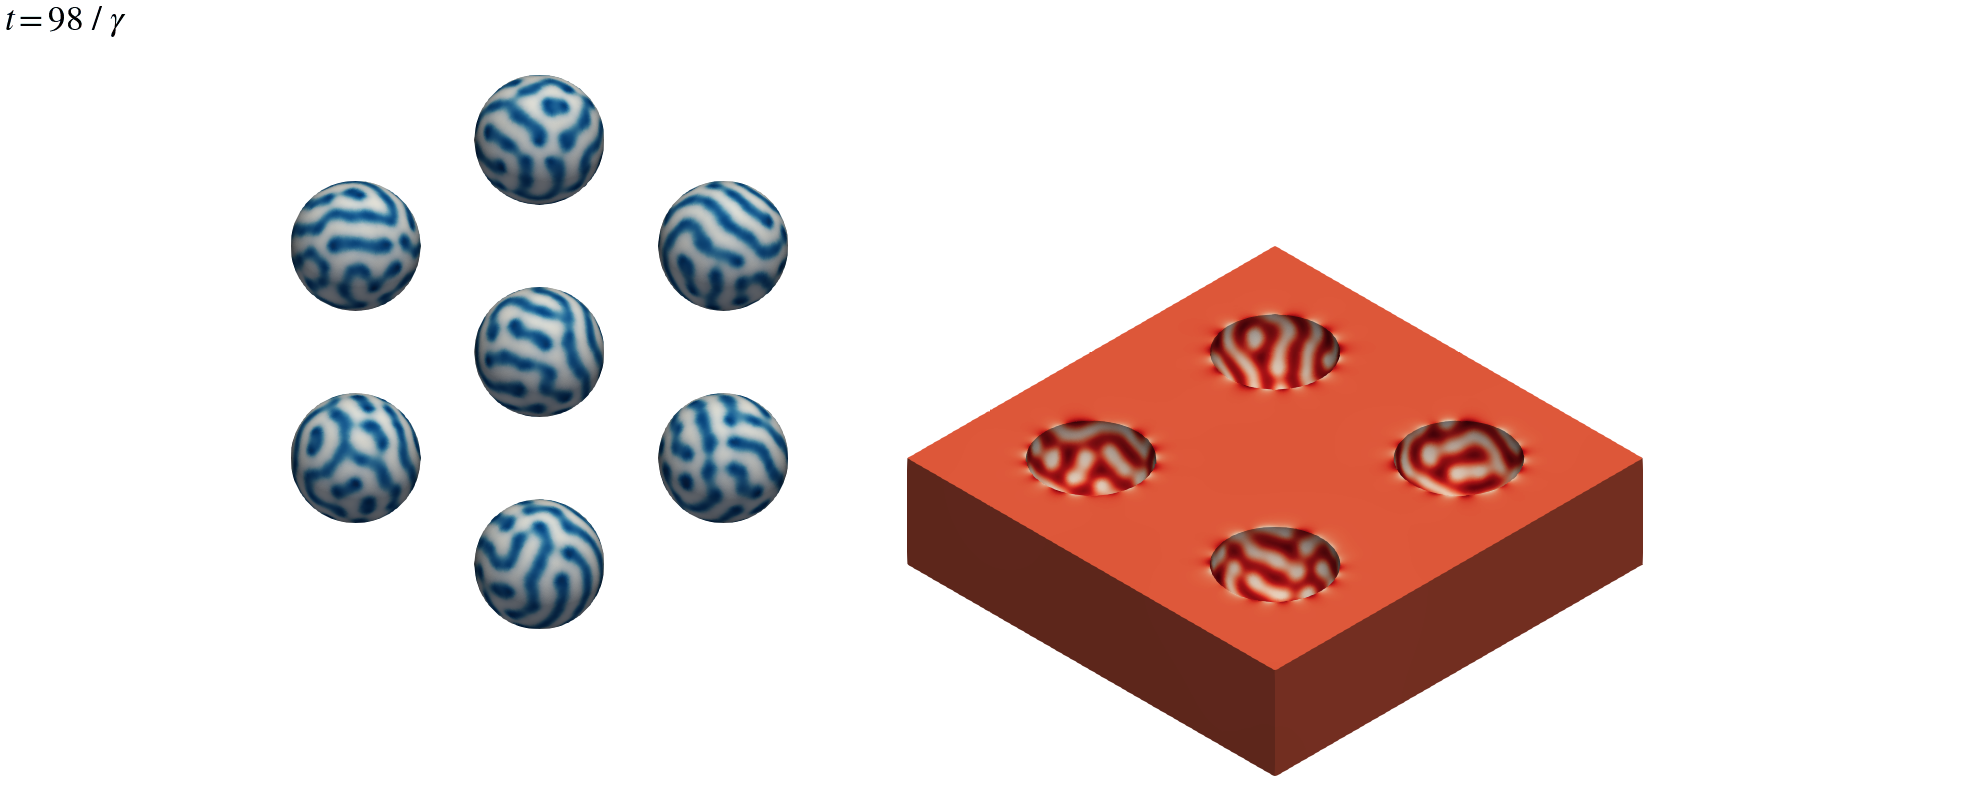
\includegraphics[width=\linewidth]{img/simulation_frames/3dbs2s_2.0128.png}
    \end{subfigure}

    \caption{A simulation of the Schnakenberg equations with extra decay for $v$ on $\Omega = (-8, 8)^2$ with $\delta_v = 0.1$, $d = 50$, $a = 0.1$, $b = 0.9$ and $\gamma = 12$. The solution is plotted for times $t = 0$, $t = 5/\gamma$ and $t = 11/\gamma$.}
    \label{fig:3d2s_3-5}
\end{figure}

\begin{figure}[t]
    \centering

    \begin{subfigure}{\textwidth}
        \centering
        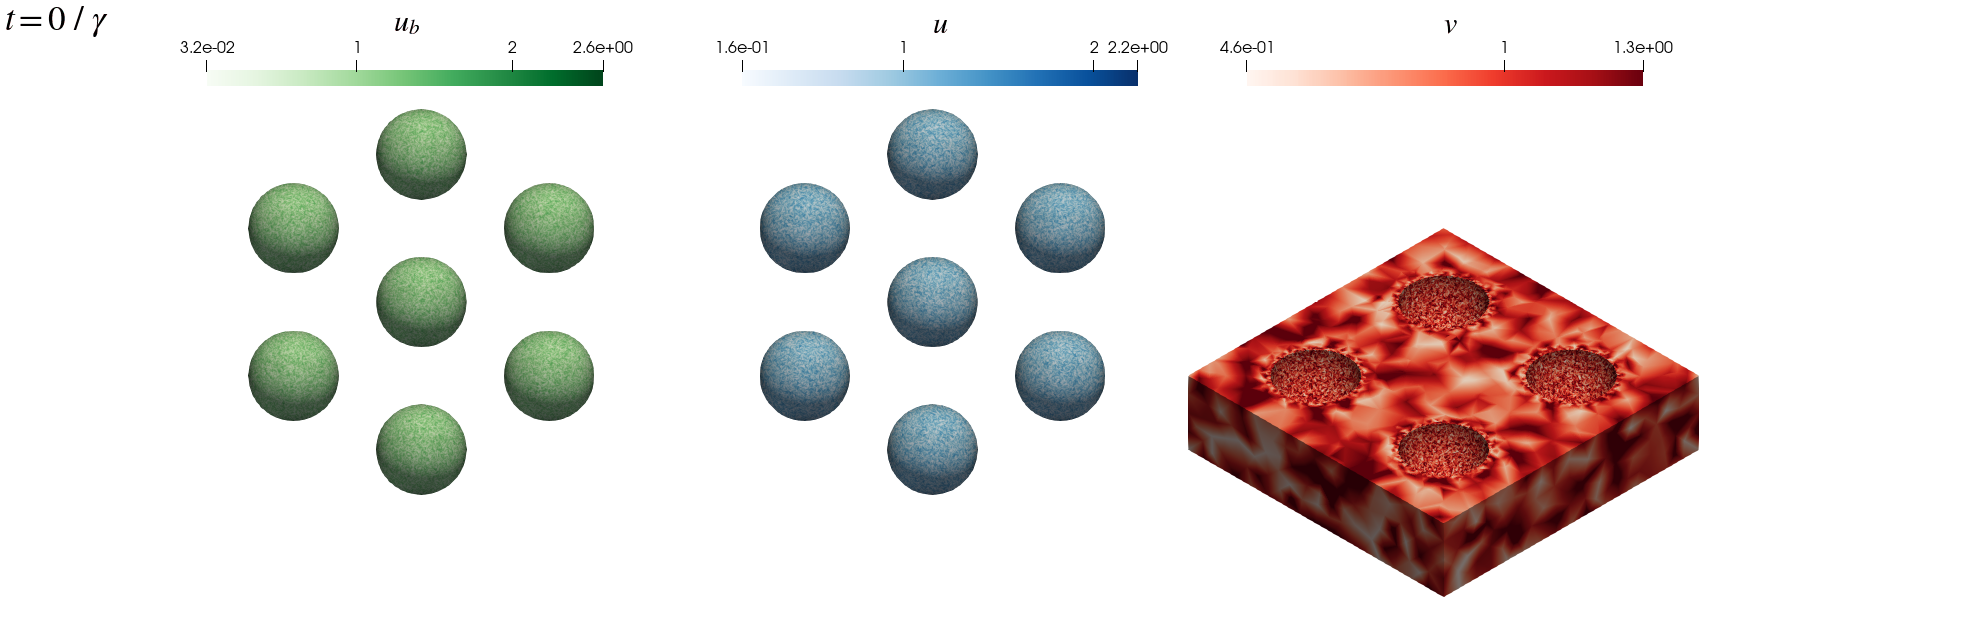
\includegraphics[width=\linewidth]{img/simulation_frames/3DBS3S.0000.png}
    \end{subfigure}

    \vspace{0.4cm}

    \begin{subfigure}{\textwidth}
        \centering
        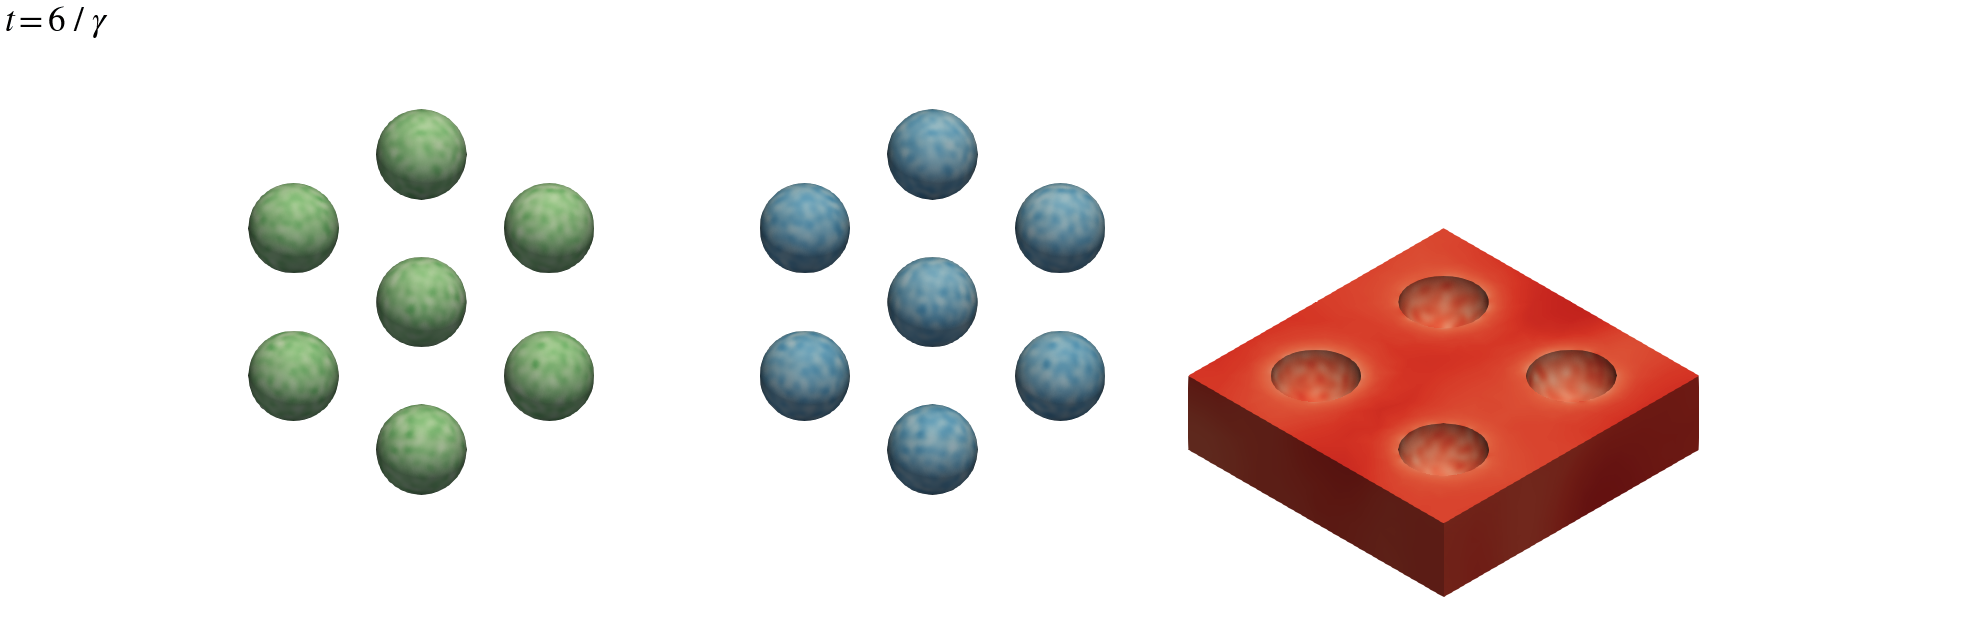
\includegraphics[width=\linewidth]{img/simulation_frames/3DBS3S.0012.png}
    \end{subfigure}

    \vspace{0.4cm}

    \begin{subfigure}{\textwidth}
        \centering
        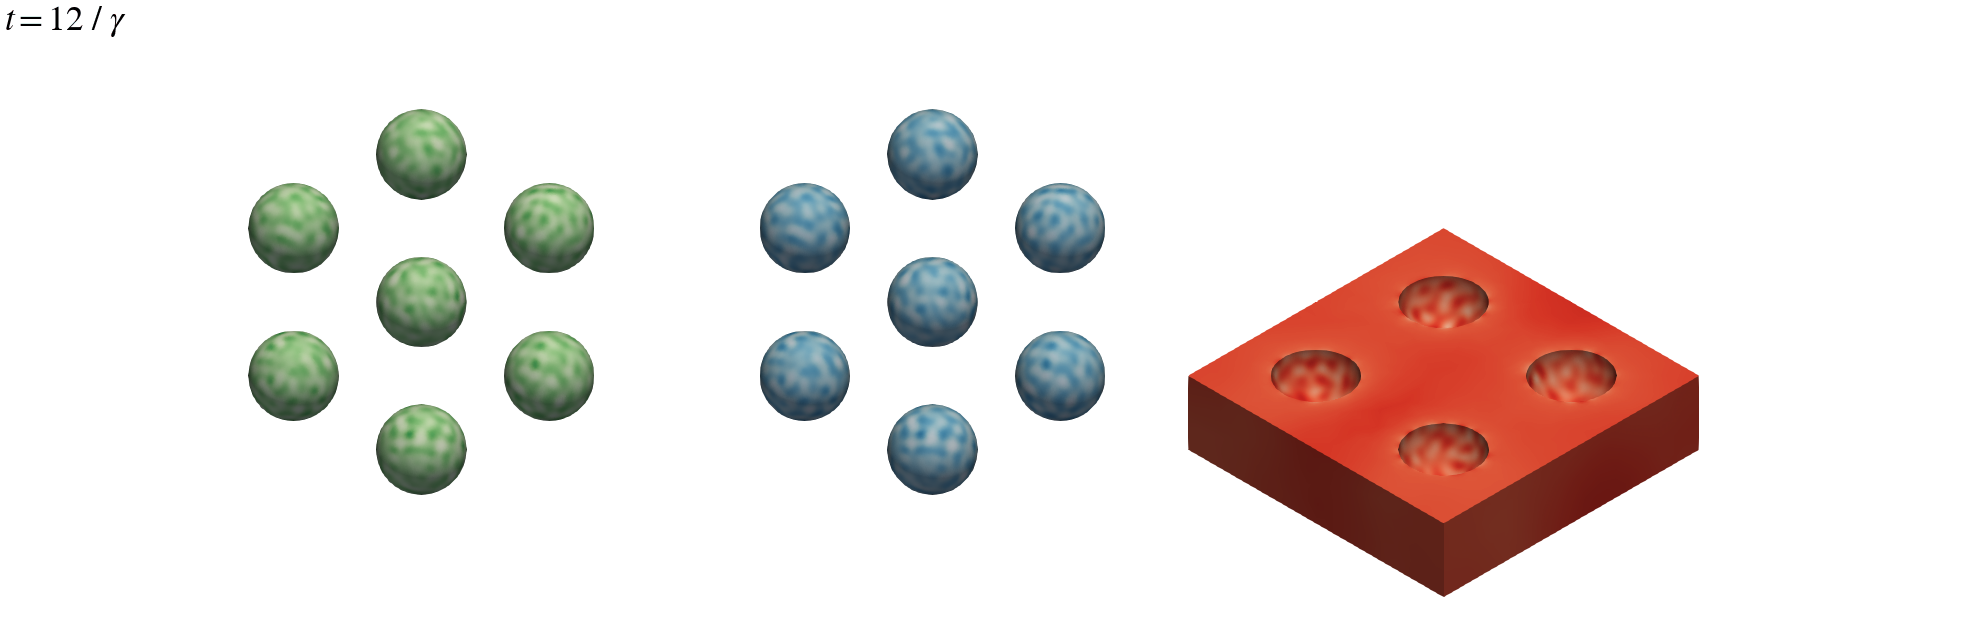
\includegraphics[width=\linewidth]{img/simulation_frames/3DBS3S.0026.png}
    \end{subfigure}

    \caption{A simulation of the Schnakenberg equations with extra decay for $v$ on $\Omega = (-8, 8)^2$ with $\delta_v = 0.1$, $d = 50$, $a = 0.1$, $b = 0.9$ and $\gamma = 12$. The solution is plotted for times $t = 0$, $t = 5/\gamma$ and $t = 11/\gamma$.}
    \label{fig:3d3s_0-2}
\end{figure}

\begin{figure}[t]
    \centering

    \begin{subfigure}{\textwidth}
        \centering
        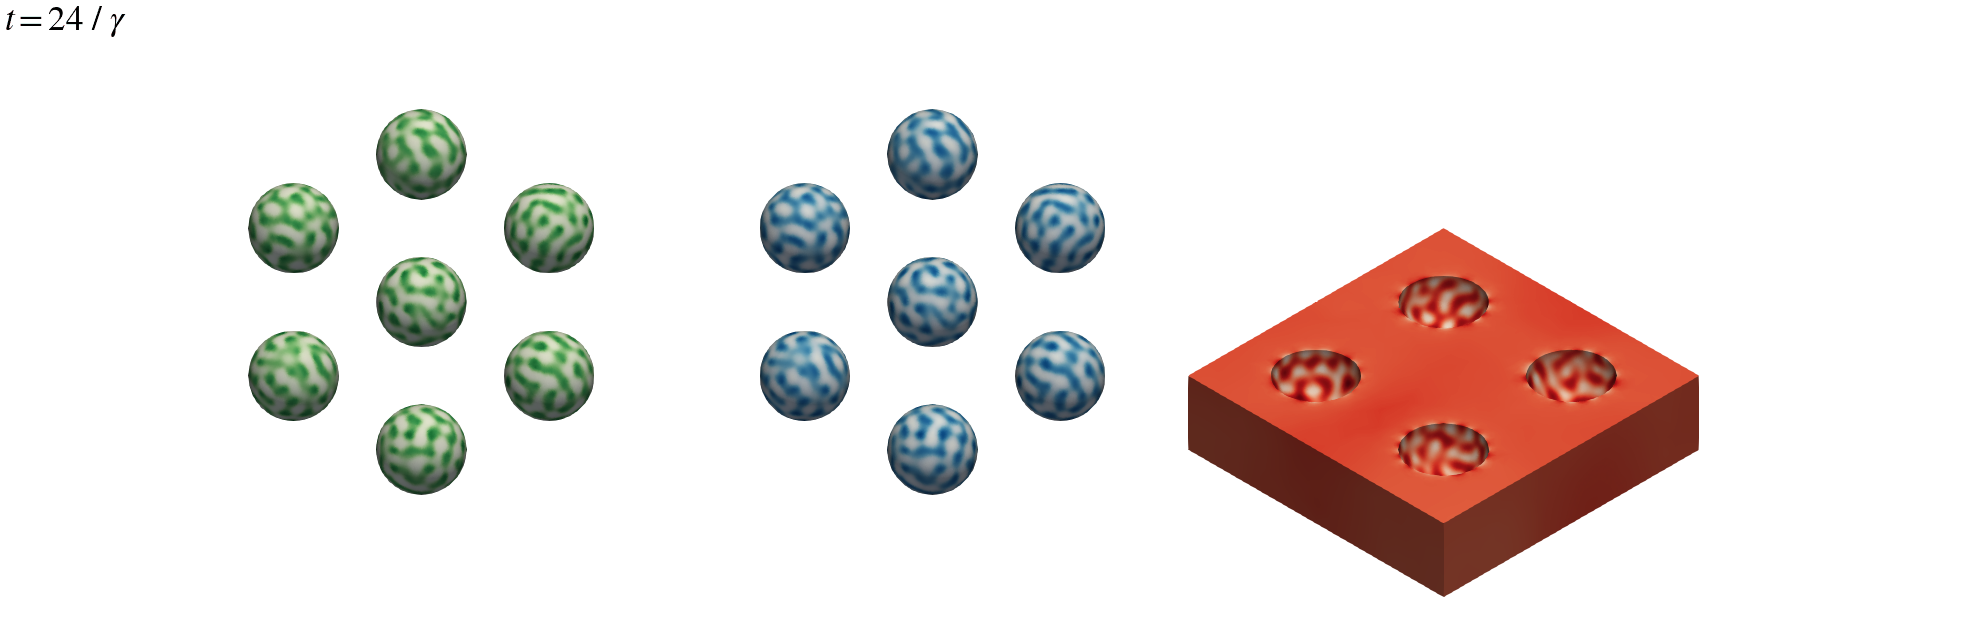
\includegraphics[width=\linewidth]{img/simulation_frames/3DBS3S.0050.png}
    \end{subfigure}

    \vspace{0.4cm}

    \begin{subfigure}{\textwidth}
        \centering
        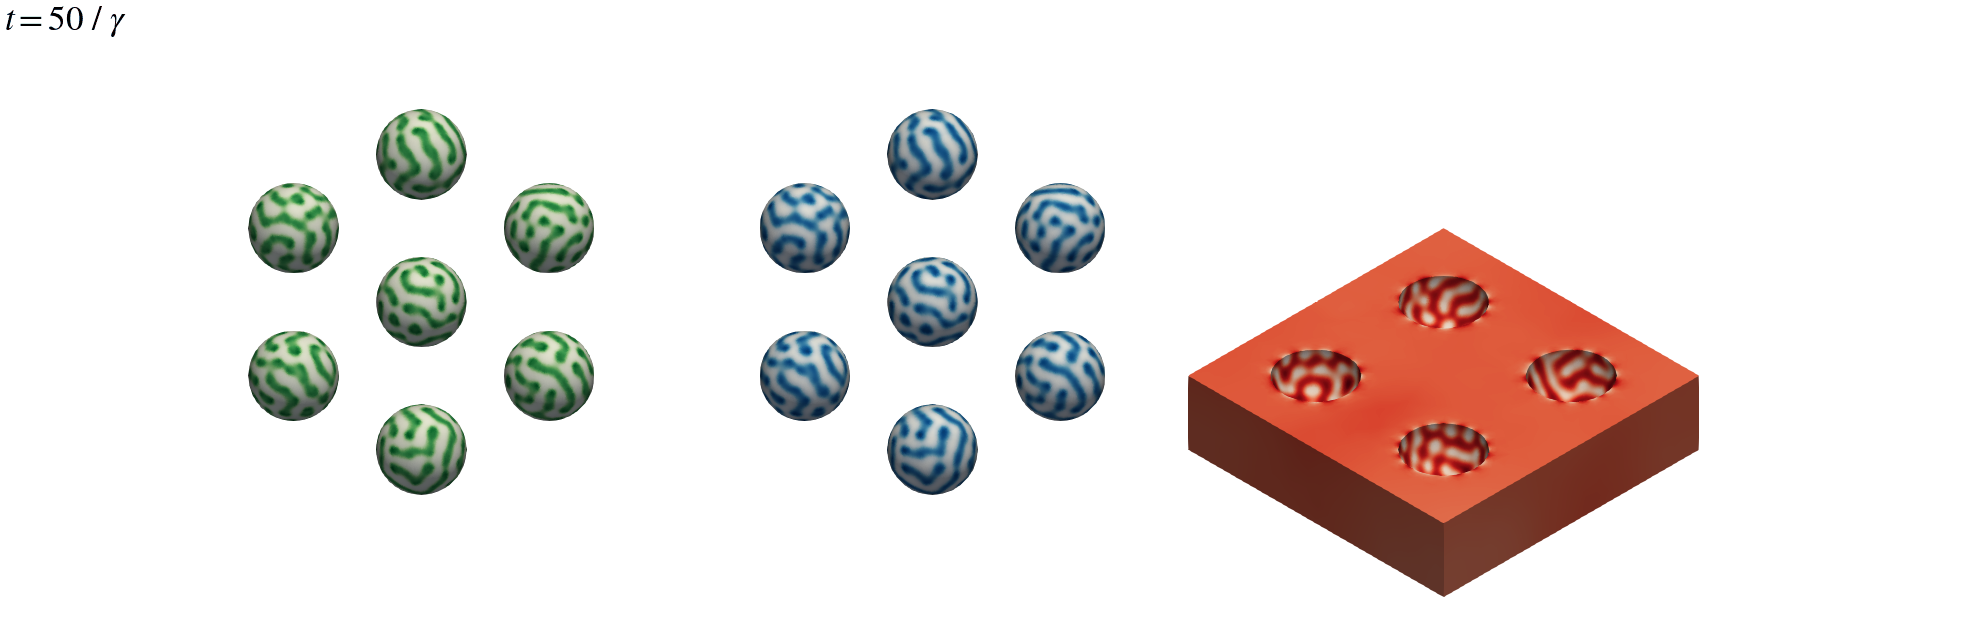
\includegraphics[width=\linewidth]{img/simulation_frames/3DBS3S.0100.png}
    \end{subfigure}

    \vspace{0.4cm}

    \begin{subfigure}{\textwidth}
        \centering
        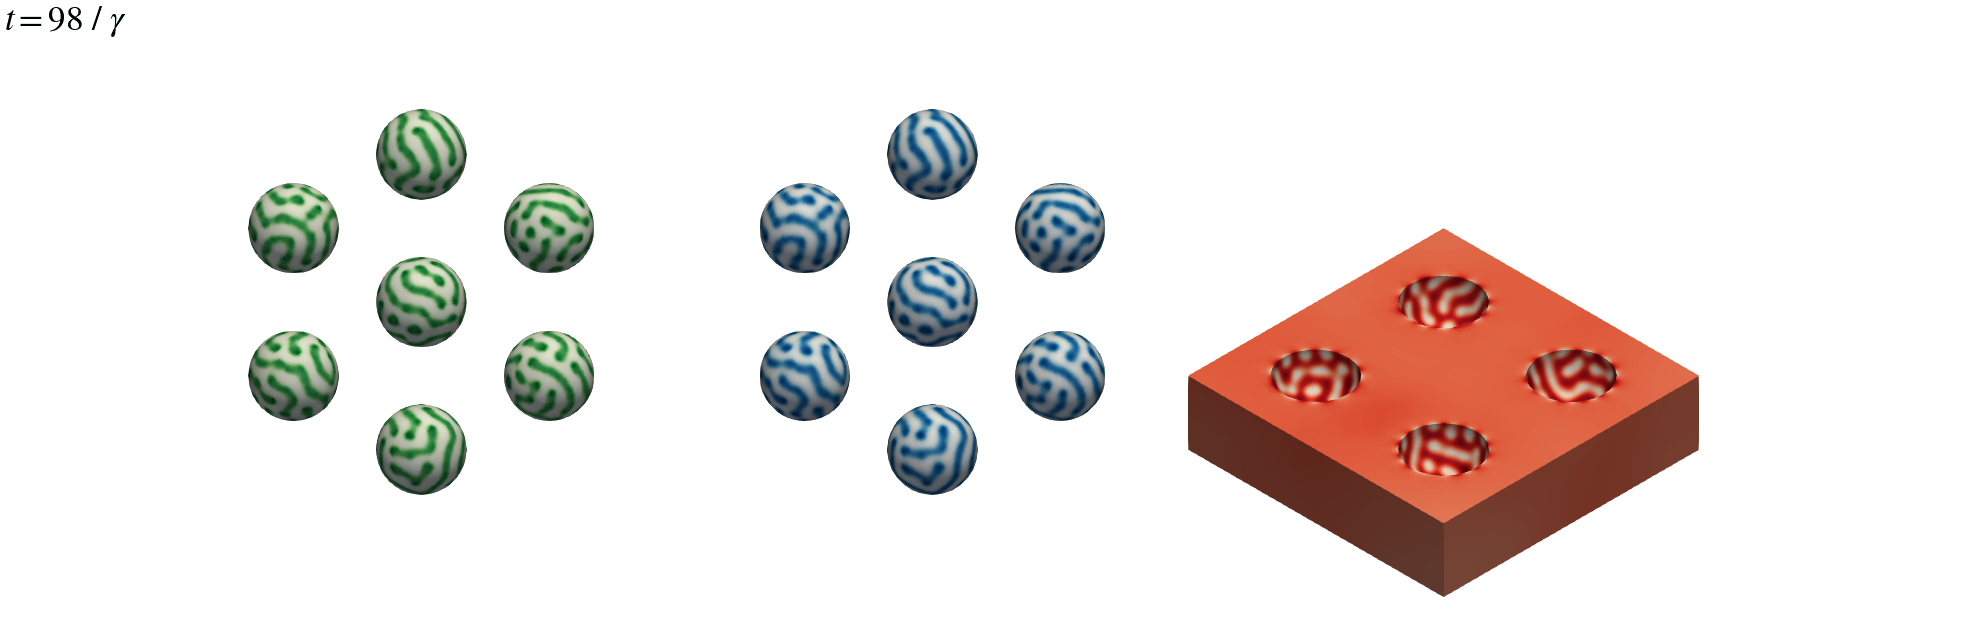
\includegraphics[width=\linewidth]{img/simulation_frames/3DBS3S.0200.png}
    \end{subfigure}

    \caption{A simulation of the Schnakenberg equations with extra decay for $v$ on $\Omega = (-8, 8)^2$ with $\delta_v = 0.1$, $d = 50$, $a = 0.1$, $b = 0.9$ and $\gamma = 12$. The solution is plotted for times $t = 0$, $t = 5/\gamma$ and $t = 11/\gamma$.}
    \label{fig:3d3s_3-5}
\end{figure}

For both $d = 2$ and $d = 3$ and the chosen parameter values, the model of \cref{eq:twospeciesmodel} seems to be a good representation for that of \cref{eq:threespeciesmodel}. Moreover, when choosing the two-species model to further study the behaviour of these PDEs, the concentration of $u_b$ can be assumed to be similar to that of $u$. These conclusions only hold for the chosen parameter values. To extend them to the general case, more tests should be done, since the parameters in \cref{eq:twospeciesmodel} leave two degrees of freedom for choosing the parameters in \cref{eq:threespeciesmodel}. Hence, every choice of parameters in \cref{eq:twospeciesmodel} admits an infinite set of parameters for \cref{eq:threespeciesmodel} such that the quasi-steady state reduction produces the same model.